\section{Concentration for $c_{\Pcal, n}(k)$ (Proving Proposition \ref{prop:concentration_local_clustering_P_n})}
\label{sec:concentration_c_P_n}

In this section we establish a concentration result for the local clustering function $c_{\Pcal, n}^\ast(k)$ in the finite model $G_{\Pcal,n}$. Similar to the previous section we will focus on those nodes $p = (x,y) \in \Kcal_{C}(k_n)$.

\subsection{The main contribution of triangles}

Recall the adjusted triangle count function \eqref{eq:def_tilde_triangle_indicator}
\[
	\widetilde{T}_{\Pcal,n}(p_0,p_1,p_2) = \ind{p_1 \in B_{\Pcal,n}(p)}\ind{p_2 \in B_{\Pcal,n}(p)}\ind{p_2 \in B_{\Pcal}(p_1) \cap \Rcal_n}.
\]
and the concentration set
\[
	\Kcal_C(k_n) = \left\{p \in \R : \frac{k_n - C \kappa_n}{\xi_{\alpha,\nu}} \vee 0 \le e^{\frac{y}{2}}
		\le \frac{k_n + C \kappa_n}{\xi_{\alpha,\nu}} \wedge e^{R_n/2} \right\},
\]
with
\[
	\kappa_n := \begin{cases}
		\log(n) &\mbox{if } k_n = \bigT{1},\\
		\sqrt{k_n \log(k_n)} &\mbox{else.}
	\end{cases}
\]
We will define the corresponding triangle degree function
\begin{equation}\label{eq:def_degree_triangle_count_in_K}
	\widetilde{T}_{\Pcal,n}(k, C) = \sum_{p \in \Pcal_n \cap K_C(k)} \ind{D_{\Pcal,n}(p) = k} \widetilde{T}_{\Pcal,n}(p),
\end{equation}
where
\[
	\widetilde{T}_{\Pcal,n}(p) := \sum_{(p_1, p_2) \in \Pcal\setminus (0,y)}^{\ne} \widetilde{T}_{\Pcal,n}(p,p_1,p_2),
\]
where the sum is over all distinct pairs $(p_1, p_2) \in \Pcal \setminus \{(0,y)\}$.

Next we note that the second result from Corollary~\ref{cor:approximation_triangle_integral} states that
\begin{equation}\label{eq:asymptotic_equivalence_contraint_triangle_count}
	\Exp{\widetilde{T}_{\Pcal,n}(k_n,C)} = (1+\smallO{1})\Exp{T_{\Pcal}(k_n)},
\end{equation}
so that we can conclude that the main contribution of triangles of degree $k_n$ is given by $\widetilde{T}_{\Pcal,n}(k_n, C)$. Therefore, in order to prove Proposition \ref{prop:concentration_local_clustering_P_n} it suffices to show that $\widetilde{T}_{\Pcal,n}(k_n,C)$ is sufficiently concentrated around its mean. This is done in the following proposition.

%\subsection{The proof of Proposition \ref{prop:concentration_local_clustering_P_n}}
%
%We start with the concentration result for $\widetilde{T}_{\Pcal,n}(k_n)$.

\begin{proposition}[Concentration $\widetilde{T}_{\Pcal,n}(k_n,C)$]\label{prop:concentration_tilde_T_P_n}
Let $\alpha > \frac{1}{2}$, $\nu > 0$ and let $(k_n)_{n \ge 1}$ be any positive sequence satisfying $k_n = \smallO{n^{\frac{1}{2\alpha+1}}}$. Then for any $C > 0$, as $n \to \infty$,
\[
	\Exp{\widetilde{T}_{\Pcal,n}(k_n,C)^2} = \left(1 + \smallO{1}\right)\Exp{\widetilde{T}_{\Pcal,n}(k_n, C)}^2.
\]
\end{proposition}

We postpone the proof of this proposition postpone till Section \ref{ssec:concentration_tilde_T} and first use it to prove Proposition \ref{prop:concentration_local_clustering_P_n}. 

%\begin{lemma}\label{lem:L1_convergence_c_Pcal_n}
%Let $\nu > 0$, $\alpha > \frac{1}{2}$ and $k_n = o\left(n^{\frac{1}{2\alpha + 1}}\right)$. Then, as $n \to \infty$,
%\[
%	\Exp{\left|c_{\Pcal, n}^\ast(k_n) - c_{\Pcal, n}(k_n)\right|} = \smallO{\Exp{c_{\Pcal,n}(k_n)^\ast}}.
%\]
%\end{lemma}
%
%\begin{proof}
%Let $0 < \delta < 1$ and define the following two events
%\begin{align*}
%	A_n &= \left\{\left|N_{\Pcal,n}(k_n) - \Exp{N_{\Pcal,n}(k_n)}\right| \le \Exp{N_{\Pcal,n}(k_n)}^{\frac{1 + \delta}{2}}\right\}\\
%	B_n &= \left\{\left|N_{\Pcal,n}(k_n) - \Exp{N_{\Pcal,n}(k_n)}\right| \le n\right\},
%\end{align*}
%so that
%\[
%	1 = \ind{A_n} + \ind{A_n^c}\ind{B_n} + \ind{B_n^c}.
%\]
%Next we note that on the event $A_n$
%\[
%	\left|\frac{\Exp{N_{\Pcal,n}(k_n)}}{N_{\Pcal,n}(k_n)} - 1\right| 
%	\le \frac{\Exp{N_{\Pcal,n}(k_n)}^{\frac{1 + \delta}{2}}}{\Exp{N_{\Pcal,n}(k_n)}+\Exp{N_{\Pcal,n}(k_n)}^{\frac{1 + \delta}{2}}}
%	\le \Exp{N_{\Pcal,n}(k_n)}^{-\frac{1 - \delta}{2}},
%\]
%and on the event $B_n$
%\[
%	\left|\frac{\Exp{N_{\Pcal,n}(k_n)}}{N_{\Pcal,n}(k_n)} - 1\right| 
%	\le \frac{n}{\Exp{N_{\Pcal,n}(k_n)} + n} \le 1.
%\]
%Therefore we have
%\begin{align*}
%	\Exp{\left|c_{\Pcal, n}^\ast(k_n) - c_{\Pcal, n}(k_n)\right|}
%	&= \Exp{c_{\Pcal, n}^\ast(k_n)\left|\frac{\Exp{N_{\Pcal,n}(k_n)}}{N_{\Pcal,n}(k_n)} - 1\right|}\\
%	&\le \Exp{c_{\Pcal, n}^\ast(k_n)\ind{A_n}}\Exp{N_{\Pcal,n}(k_n)}^{-\frac{1 - \delta}{2}} \\
%	&\hspace{10pt}+ \Exp{c_{\Pcal, n}^\ast(k_n)\ind{A_n^c}\ind{B_n}} \\
%	&\hspace{10pt}+ \Exp{c_{\Pcal, n}^\ast(k_n)\left|\frac{\Exp{N_{\Pcal,n}(k_n)}}{N_{\Pcal,n}(k_n)} - 1\right|\ind{B_n^c}}
%\end{align*}
%Since $\Exp{N_{\Pcal,n}(k_n)} \to \infty$, the first term is clearly $\smallO{\Exp{c_{\Pcal, n}^\ast(k_n)}}$. For the third term we have
%\begin{align*}
%	\Exp{c_{\Pcal, n}^\ast(k_n)\left|\frac{\Exp{N_{\Pcal,n}(k_n)}}{N_{\Pcal,n}(k_n)} - 1\right|\ind{B_n^c}} 
%	&= \bigO{\Prob{B_n^c}}
%		= \bigO{\Prob{\left|N_{\Pcal,n}(k_n) - \Exp{N_{\Pcal,n}(k_n)}\right| > n}}\\
%	&= \bigO{e^{-\frac{n^2}{\Exp{N_{k_n}} + n}}} = \bigO{e^{-n}} = \smallO{\Exp{c_{\Pcal, n}^\ast(k_n)}}.
%\end{align*}
%Hence we are left to show that
%\begin{equation}\label{eq:L1_convergence_second_term}
%	\Exp{c_{\Pcal, n}^\ast(k_n)\ind{A_n^c}\ind{B_n}} = \smallO{\Exp{c_{\Pcal, n}^\ast(k_n)}}.
%\end{equation}
%By writing
%\begin{align*}
%	c_{\Pcal, n}^\ast(k_n) = \frac{\widetilde{T}_{\Pcal,n}(k_n,\varepsilon)}{\binom{k_n}{2}\Exp{N_{\Pcal,n}(k_n)}}
%	+ \frac{T_{\Pcal,n}(k_n,\varepsilon)- \widetilde{T}_{\Pcal,n}(k_n,\varepsilon)}{\binom{k_n}{2}\Exp{N_{\Pcal,n}(k_n)}}
%\end{align*}
%and using Lemma~\ref{lem:clustering_error_T_term} we get
%\begin{align*}
%	\Exp{c_{\Pcal, n}^\ast(k_n)\ind{A_n^c}\ind{B_n}}
%	&\le \Exp{\frac{(1+\smallO{1})\widetilde{T}_{\Pcal,n}(k_n,\varepsilon)}{\binom{k_n}{2}\Exp{N_{\Pcal,n}(k_n)}}
%		\ind{A_n^c}} + \smallO{\Exp{c_{\Pcal, n}^\ast(k_n)}}.
%\end{align*}
%For the last step we use H\"{o}lder's inequality and Proposition \ref{prop:concentration_tilde_T_P_n} to get
%\begin{align*}
%	\Exp{\frac{\widetilde{T}_{\Pcal,n}(k_n,\varepsilon)}{\binom{k_n}{2}\Exp{N_{\Pcal,n}(k_n)}}\ind{A_n^c}}
%	&\le \Exp{\left(\frac{\widetilde{T}_{\Pcal,n}(k_n,\varepsilon)}
%		{\binom{k_n}{2}\Exp{N_{\Pcal,n}(k_n)}}\right)^2}^{\frac{1}{2}} \Prob{A_n^c}^{\frac{1}{2}}\\
%	&= \left(1 + \smallO{1}\right) 	
%		\frac{\Exp{\widetilde{T}_{\Pcal,n}(k_n,\varepsilon)}}{\binom{k_n}{2}\Exp{N_{\Pcal,n}(k_n)}}
%		\Prob{A_n^c}^{\frac{1}{2}}\\
%	&= \bigO{\Exp{c_{\Pcal, n}^\ast(k_n)}}\Prob{A_n^c}^{\frac{1}{2}} = \smallO{\Exp{c_{\Pcal, n}^\ast(k_n)}},
%\end{align*}
%since $\Prob{A_n} = o(1)$. This establishes \eqref{eq:L1_convergence_second_term} and hence we conclude that
%\[
%	\Exp{\left|c_{\Pcal, n}^\ast(k_n) - c_{\Pcal, n}(k_n)\right|} = \smallO{\Exp{c_{\Pcal,n}(k_n)^\ast}}.
%\]
%\end{proof}

\begin{proof}[Proof of Proposition \ref{prop:concentration_local_clustering_P_n}]
Again, we write
\begin{align*}
	c_{\Pcal, n}^\ast(k_n) = \frac{\widetilde{T}_{\Pcal,n}(k_n,C)}{\binom{k_n}{2}\Exp{N_{\Pcal,n}(k_n)}}
	+ \frac{\left(T_{\Pcal,n}(k_n)-\widetilde{T}_{\Pcal,n}(k_n,C)\right)}{\binom{k_n}{2}\Exp{N_{\Pcal,n}(k_n)}},
\end{align*}
so that by~\eqref{eq:asymptotic_equivalence_contraint_triangle_count},
\begin{equation}\label{eq:concentration_local_clustering_P_n_main}
	\Exp{c_{\Pcal,n}^\ast(k_n)} = \frac{\Exp{\widetilde{T}_{\Pcal,n}(k_n,C)}}{\binom{k_n}{2}\Exp{N_{\Pcal,n}(k_n)}}
	+ \smallO{\Exp{c_{\Pcal,n}^\ast(k_n)}}.
\end{equation}
%Therefore, by Lemma \ref{lem:L1_convergence_c_Pcal_n},
%\begin{align*}
%	\Exp{\left|c_{\Pcal,n}(k_n) - \Exp{c_{\Pcal,n}^\ast(k_n)}\right|}
%	&\le \Exp{\left|c_{\Pcal,n}^\ast(k_n) - \Exp{c_{\Pcal,n}^\ast(k_n)}\right|}
%		+ \Exp{\left|c_{\Pcal,n}(k_n) - c_{\Pcal,n}^\ast(k_n)\right|}\\
%	&= \frac{\Exp{\left|\widetilde{T}_{\Pcal,n}(k_n,\varepsilon) - \Exp{\widetilde{T}_{\Pcal,n}(k_n,\varepsilon)}\right|}}
%		{\binom{k_n}{2}\Exp{N_{\Pcal,n}(k_n)}} + \smallO{\Exp{c_{\Pcal,n}^\ast(k_n)}}.
%		\numberthis \label{eq:concentration_local_clustering_P_n_term1}
%\end{align*}
Next, we use Proposition \ref{prop:concentration_tilde_T_P_n} to obtain
\begin{align*}
	\Exp{\left|\widetilde{T}_{\Pcal,n}(k_n,C) - \Exp{\widetilde{T}_{\Pcal,n}(k_n,C)}\right|}
	&\le \left(\Exp{\widetilde{T}_{\Pcal,n}(k_n,C)^2} 
		- \Exp{\widetilde{T}_{\Pcal,n}(k_n,C)}^2\right)^{\frac{1}{2}}\\
	&= \smallO{\Exp{\widetilde{T}_{\Pcal,n}(k_n,C)}}.
\end{align*}
This implies
\begin{align*}
	\frac{\Exp{\left|\widetilde{T}_{\Pcal,n}(k_n,\varepsilon) - \Exp{\widetilde{T}_{\Pcal,n}(k_n,\varepsilon)}\right|}}
		{\binom{k_n}{2}\Exp{N_{\Pcal,n}(k_n)}}
	&= \smallO{\Exp{c_{\Pcal,n}^\ast(k_n)}},
\end{align*}
which together with~\eqref{eq:concentration_local_clustering_P_n_main} yields the required result.
\end{proof}

\subsection{Joint neighborhoods and degrees in $G_{\Pcal,n}(\alpha,\nu)$}

To prove Proposition~\ref{prop:concentration_tilde_T_P_n} we need to understand the joint degree distribution in $G_{\Pcal,n}$ and subsequently the joint neighborhoods of two points $p, p^\prime \in \Rcal_n$. We perform the analysis in this section. The two main results, which will be the crucial technical ingredients for the proof of Proposition~\ref{prop:concentration_tilde_T_P_n}, are Lemma ?? and Lemma ??.

\subsubsection*{Neighborhoods}

We start with analyzing joint neighborhoods in $G_{\Pcal,n}$. Let $p, p^\prime \in \Rcal_n$. Then we denote by $\Ncal_{\Pcal,n}(p\Delta p^\prime)$ the number of disjoint neighbors of $p$ and $p^\prime$ in $G_{\Pcal,n}$, i.e. those points that belong to either $\BallPon{p}$ or $\BallPon{p^\prime}$ but not to their intersection. In addition we denote by $\Ncal_{\Pcal,n}(p,p^\prime)$ the number of joint neighbors of $p$ and $p^\prime$. We shall establish lower bounds on the expect number of these disjoint neighbors $\Exp{\Ncal_{\Pcal,n}(p\Delta p^\prime)}$ as well as an asymptotic expression for the expected number of joint neighbors. For this we will distinguish between the cases where the distance between the $x$-coordinates of $p$ and $p^\prime$ is small or large. Figure~\ref{fig:representation_disjoint_neighborhoods_P_n}-\ref{fig:representation_disjoint_neighborhoods_P_n_3} show the different situations that occur.

\begin{figure}[p]
\centering
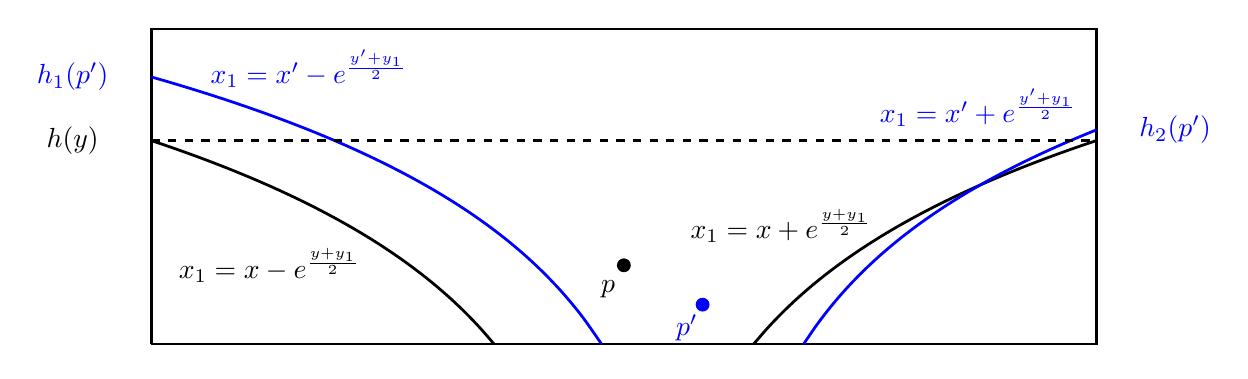
\begin{tikzpicture}
	
	%The box \Rcal_n
	\draw[line width=1pt] (-6,0) -- (6,0) -- (6,4) -- (-6,4) -- (-6,0);

    \draw node[fill, circle, inner sep=0pt, minimum size=5pt] at (0,1) {};
    \draw node at (-0.2,0.7) {$p$};
    
    \draw node[fill,blue, circle, inner sep=0pt, minimum size=5pt] at (1,0.5) {};
    \draw node at (0.8,0.2) {\color{blue}$p^\prime$};
	
	\draw[domain=1.6487:6,smooth,variable=\x,black,line width=1pt] plot (\x, {2*ln(\x)-1});
    \draw[domain=-1.6487:-6,smooth,variable=\x,black,line width=1pt] plot (\x, {2*ln(-\x)-1});
    \draw[domain=2.2840:6,smooth,variable=\x,blue,line width=1pt] plot (\x, {2*ln(\x-1)-0.5});
    \draw[domain=-0.2840:-6,smooth,variable=\x,blue,line width=1pt] plot (\x, {2*ln(1-\x)-0.5});
    
    \draw[dashed,thick,black,line width=1pt] (-6,2.5835) -- (6,2.5835);
    
    \draw node at (-7,2.5835) {$h(y)$};
    \draw node at (-7,3.3918) {\color{blue}$h_1(p^\prime)$};
    \draw node at (7,2.7189) {\color{blue}$h_2(p^\prime)$};
    
    \draw node at (-4,3.5) {\color{blue}$x_1 = x^\prime - e^{\frac{y^\prime + y_1}{2}}$};
    \draw node at (4.5,3) {\color{blue}$x_1 = x^\prime + e^{\frac{y^\prime + y_1}{2}}$};
    \draw node at (-4.5,1) {$x_1 = x - e^{\frac{y + y_1}{2}}$};
    \draw node at (2,1.5) {$x_1 = x + e^{\frac{y + y_1}{2}}$};

\end{tikzpicture}
\caption{Schematic representation of the neighborhoods of $p$ and $p^\prime$ in $G_{\Pcal,n}(\alpha,\nu)$ when $|x-x^\prime| \le e^{\frac{y + y^\prime}{2}}$ used for the proof of Lemma~\ref{lem:disjoint_neighbors_P_n} and Lemma~\ref{lem:common_neighbors_Pcal_n}.}
\label{fig:representation_disjoint_neighborhoods_P_n}
\end{figure}~
\begin{figure}[p]
\centering
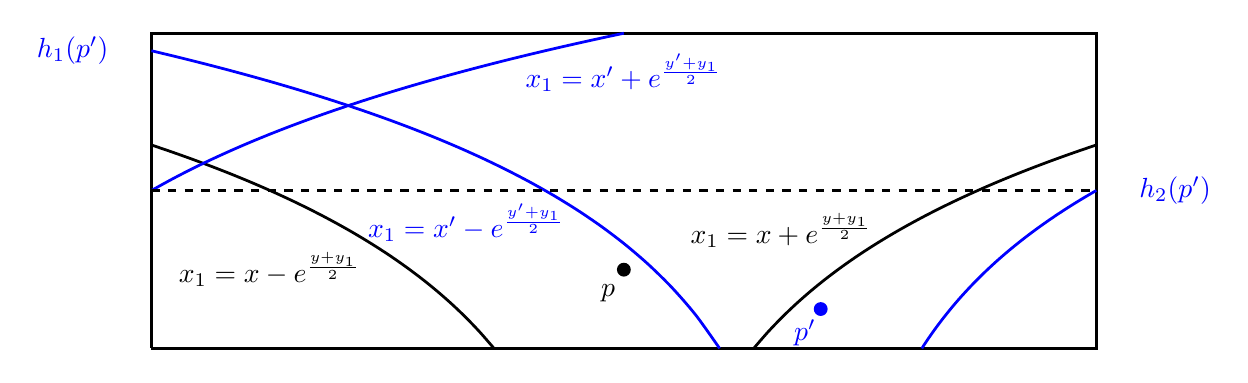
\begin{tikzpicture}
	
	%The box \Rcal_n
	\draw[line width=1pt] (-6,0) -- (6,0) -- (6,4) -- (-6,4) -- (-6,0);

    \draw node[fill, circle, inner sep=0pt, minimum size=5pt] at (0,1) {};
    \draw node at (-0.2,0.7) {$p$};
    
    \draw node[fill,blue, circle, inner sep=0pt, minimum size=5pt] at (2.5,0.5) {};
    \draw node at (2.3,0.2) {\color{blue}$p^\prime$};
	
	\draw[domain=1.6487:6,smooth,variable=\x,black,line width=1pt] plot (\x, {2*ln(\x)-1});
    \draw[domain=-1.6487:-6,smooth,variable=\x,black,line width=1pt] plot (\x, {2*ln(-\x)-1});
    \draw[domain=3.7840:6,smooth,variable=\x,blue,line width=1pt] plot (\x, {2*ln(\x-2.5)-0.5});
    \draw[domain=1.2160:-6,smooth,variable=\x,blue,line width=1pt] plot (\x, {2*ln(2.5-\x)-0.5});
    \draw[domain=0:-6,smooth,variable=\x,blue,line width=1pt] plot (\x, {2*ln(\x+9.5)-0.5});
    
    \draw[dashed,black,line width=1pt] (-6,2.0055) -- (6,2.0055);
    
%    \draw node at (-7,2.5835) {$h(y)$};
    \draw node at (-7,3.7801) {\color{blue}$h_1(p^\prime)$};
    \draw node at (7,2.0055) {\color{blue}$h_2(p^\prime)$};
    
%    \draw[dotted,thick,black] (4.5208,2.0174) -- (4.5208,0);
%    \draw[dotted,thick,black] (4.5208,2.0174) -- (6,2.0174);
    
%    \draw node at (4.5208,-0.5) {$w_x(p,p^\prime)$};
%    \draw node at (7,2.0174) {$w_y(p,p^\prime)$};
    
    \draw node at (0,3.5) {\color{blue}$x_1 = x^\prime + e^{\frac{y^\prime + y_1}{2}}$};
    \draw node at (-2,1.6) {\color{blue}$x_1 = x^\prime - e^{\frac{y^\prime + y_1}{2}}$};
    \draw node at (-4.5,1) {$x_1 = x - e^{\frac{y + y_1}{2}}$};
    \draw node at (2,1.5) {$x_1 = x + e^{\frac{y + y_1}{2}}$};

\end{tikzpicture}
\caption{Schematic representation of the neighborhoods of $p$ and $p^\prime$ in $G_{\Pcal,n}(\alpha,\nu)$ when $e^{\frac{y + y^\prime}{2}} < |x - x^\prime| \le e^{\frac{y}{2}} + e^{\frac{y^\prime}{2}}$ used for the proof of Lemma~\ref{lem:disjoint_neighbors_P_n} and Lemma~\ref{lem:common_neighbors_Pcal_n}.}
\label{fig:representation_disjoint_neighborhoods_P_n_2}
\end{figure}~
\begin{figure}[p]
\centering
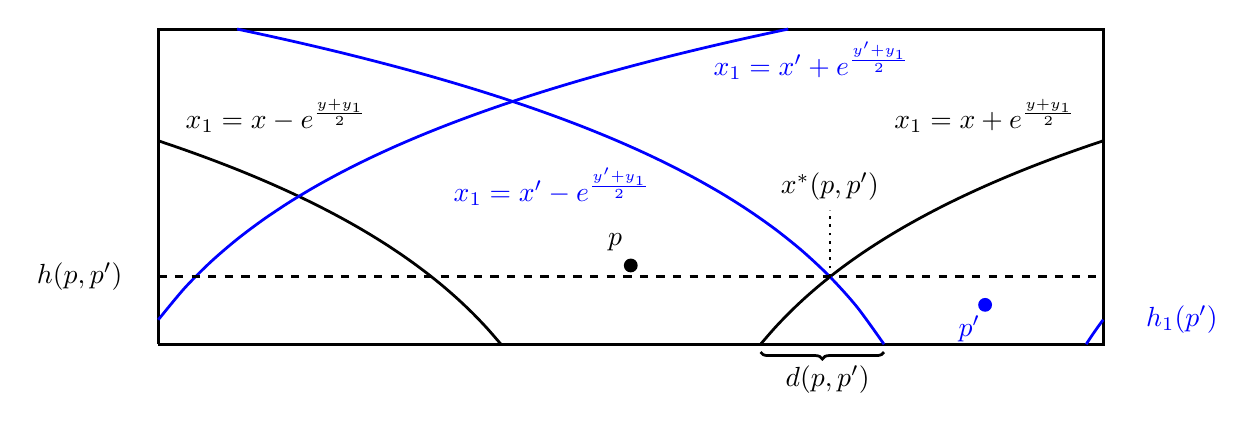
\begin{tikzpicture}
	
	%The box \Rcal_n
	\draw[line width=1pt] (-6,0) -- (6,0) -- (6,4) -- (-6,4) -- (-6,0);

    \draw node[fill, circle, inner sep=0pt, minimum size=5pt] at (0,1) {};
    \draw node at (-0.2,1.3) {$p$};
    
    \draw node[fill,blue, circle, inner sep=0pt, minimum size=5pt] at (4.5,0.5) {};
    \draw node at (4.3,0.2) {\color{blue}$p^\prime$};
	
	\draw[domain=1.6487:6,smooth,variable=\x,black,line width=1pt] plot (\x, {2*ln(\x)-1});
    \draw[domain=-1.6487:-6,smooth,variable=\x,black,line width=1pt] plot (\x, {2*ln(-\x)-1});
    \draw[domain=5.7840:6,smooth,variable=\x,blue,line width=1pt] plot (\x, {2*ln(\x-4.5)-0.5});
    \draw[domain=3.2160:-5,smooth,variable=\x,blue,line width=1pt] plot (\x, {2*ln(4.5-\x)-0.5});
    \draw[domain=2:-6,smooth,variable=\x,blue,line width=1pt] plot (\x, {2*ln(\x+7.5)-0.5});
    
    \draw[dashed,black,line width=1pt] (-6,0.8563) -- (6,0.8563);
    
    \draw node at (-7,0.8563) {$h(p,p^\prime)$};
    \draw node at (7,0.3109) {\color{blue}$h_1(p^\prime)$};
    
    \draw [decorate,decoration={brace},line width=1pt] (3.2160,-0.1) -- (1.6487,-0.1);
    \draw node at (2.5,-0.45) {$d(p,p^\prime)$};
    
    \draw [dotted,line width=1pt] (2.5298,0.8563) -- (2.5298,1.7);
    \draw node at (2.5298,2) {$x^\ast(p,p^\prime)$};
    
%    \draw[dotted,thick,black] (4.5208,2.0174) -- (4.5208,0);
%    \draw[dotted,thick,black] (4.5208,2.0174) -- (6,2.0174);
    
%    \draw node at (4.5208,-0.5) {$w_x(p,p^\prime)$};
%    \draw node at (7,2.0174) {$w_y(p,p^\prime)$};
    
    \draw node at (2.3,3.6) {\color{blue}$x_1 = x^\prime + e^{\frac{y^\prime + y_1}{2}}$};
    \draw node at (-1,2) {\color{blue}$x_1 = x^\prime - e^{\frac{y^\prime + y_1}{2}}$};
    \draw node at (-4.5,2.9) {$x_1 = x - e^{\frac{y + y_1}{2}}$};
    \draw node at (4.5,2.9) {$x_1 = x + e^{\frac{y + y_1}{2}}$};

\end{tikzpicture}
\caption{Schematic representation of the neighborhoods of $p$ and $p^\prime$ in $G_{\Pcal,n}(\alpha,\nu)$ when $|x - x^\prime| > e^{\frac{y}{2}} + e^{\frac{y^\prime}{2}}$ used for the proof of Lemma \ref{lem:disjoint_neighbors_P_n_large}.}
\label{fig:representation_disjoint_neighborhoods_P_n_3}
\end{figure}


We start by analyzing the shape of the neighborhoods. Due to symmetry and the fact that we have identified the left and right boundaries of the box $\Rcal_n$, we can, without loss of generality, assume that $p = (0,y)$ and $p^\prime = (x^\prime,y^\prime)$ with $x^\prime > 0$ and $y^\prime \le y$. To understand the computation it is helpful to have a picture of the different situations. Figure \ref{fig:representation_disjoint_neighborhoods_P_n} and Figure \ref{fig:representation_disjoint_neighborhoods_P_n_2} show two different situations for small distance in the $x$-coordinates, in which case the number of disjoint neighbors is small. The case where this distance is large, and the number of disjoint neighbors is expected to be large, is show in Figure \ref{fig:representation_disjoint_neighborhoods_P_n_3}. There are several different quantities that are important. The first are the heights $h_1(p^\prime)$ and $h_2(p^\prime)$ where, respectively, the left and right boundaries of the ball $\BallPon{p^\prime}$ go outside the box $\Rcal_n$. Note that when $x = 0$ then these height are the same and we denote this by $h(y)$. We also need to know the coordinates $h(p,p^\prime)$ and $x^\ast(p,p^\prime)$ of the intersection of the right boundary of the neighborhood of $p$ with the left boundary of the neighborhood of $p^\prime$. Finally we will denote by $d(p,p^\prime)$ the distance between the lower right boundary of $\BallPon{p}$ and the lower left of $\BallPon{p^\prime}$, which is positive only when the bottom parts of both neighborhoods do not intersect, compare Figures \ref{fig:representation_disjoint_neighborhoods_P_n} and \ref{fig:representation_disjoint_neighborhoods_P_n_3}. The full expressions of all these functions are given below for further reference.

\begin{align}
	h(y) &= R_n - y + 2\log\left(\frac{\pi}{2}\right) \label{eq:def_height_y_P_n}\\
	h_1(p^\prime) &= 2\log\left(x^\prime + \frac{\pi}{2}e^{\frac{R_n}{2}}\right) - y^\prime \label{eq:def_height_left_P_n} \\
	h_2(p^\prime) &= 2\log\left(\frac{\pi}{2}e^{\frac{R_n}{2}} - x^\prime\right) - y^\prime 
		\label{eq:def_height_right_P_n} \\
%	\iota_x(p,p^\prime) &= \frac{(x^\prime-x)e^{\frac{y}{2}}}{e^{\frac{y}{2}} - e^{\frac{y^\prime}{2}}}
%		\label{eq:def_x_intersection_close_boundaries}\\
%	\iota_y(p,p^\prime) &= 2\log\left(\frac{x^\prime - x}{e^{\frac{y}{2}} - e^{\frac{y^\prime}{2}}}\right)
%		\label{eq:def_y_intersection_close_boundaries}\\
	h((p,p^\prime) &= 2\log\left(\frac{|x - x^\prime|}{e^{\frac{y}{2}} + e^{\frac{y^\prime}{2}}}\right)\\
	x^\ast(p,p^\prime) &= \frac{x e^{\frac{y^\prime}{2}} + x^\prime e^{\frac{y}{2}}}{e^{\frac{y}{2}} + 	
		e^{\frac{y^\prime}{2}}},\\
	d(p,p^\prime) &= |x - x^\prime| - \left(e^{\frac{y}{2}} + e^{\frac{y^\prime}{2}}\right).
	\label{eq:def_d_p_p_prime}
\end{align}

We start with the result for points whose $x$-coordinates are close, which is when $d(p,p^\prime) < 0$.

\begin{lemma}\label{lem:disjoint_neighbors_P_n}
Let $p, p ^\prime \in \Rcal_n$. Then whenever $|x - x^\prime| \le e^{\frac{y}{2}} + e^{\frac{y^\prime}{2}}$,
\begin{align*}
	\Exp{\Ncal_{\Pcal,n}(p \Delta p^\prime)}
	&\ge \frac{\nu}{\pi}|x^\prime - x|\left(1 - \left(\frac{2}{\pi}\right)^{2\alpha}e^{-\alpha(R_n - y^\ast)}\right)\\
	&\hspace{10pt}+ \xi_{\alpha, \nu}\left|e^{\frac{y}{2}} - e^{\frac{y^\prime}{2}}\right|
		\left(1 - \left(\frac{2}{\pi}\right)^{2\alpha - 1}e^{-(\alpha - \frac{1}{2})(R_n-y^\ast)}\right).
\end{align*}
\end{lemma}

\begin{proof}
In order to proof the result we will consider the area in between the two left boundaries of the balls $\BallPon{p}$ and
$\BallPon{p^\prime}$ up to the height $h^\ast := \min\{h(y), h_2(p^\prime)\}$, see Figure~\ref{fig:representation_disjoint_neighborhoods_P_n} and Figure~\ref{fig:representation_disjoint_neighborhoods_P_n_2} for reference. Note that here we do not need to consider different cases depending on whether $|x - x^\prime| \le e^{(y + y^\prime)/2}$ or $|x - x^\prime| > e^{(y + y^\prime)/2}$. 

By the Campbell-Mecke formula we get
\begin{align*}
	\Exp{\Ncal_{\Pcal,n}(p \Delta p^\prime)} &=	\Mu{B_{\Pcal,n}(p) \Delta B_{\Pcal,n}(p^\prime)}\\
	&\ge \int_0^{h^\ast} \int_{x - e^{\frac{y + y_1}{2}}}^{x^\prime - e^{\frac{y^\prime + y_1}{2}}} f_{\alpha,\nu}(x_1,y_1)
		\, dx_1 \, dy_1 \\
	&= \frac{\alpha \nu}{\pi}|x^\prime - x| \int_{0}^{h^\ast} e^{-\alpha y_1} dy_1
		+ \frac{\alpha \nu}{\pi}\left|e^{\frac{y}{2}} - e^{\frac{y^\prime}{2}}\right| \int_0^{h^\ast} 
		e^{-(\alpha-\frac{1}{2})y_1} \, dy_1\\
	&= \frac{\nu}{\pi}|x^\prime - x|\left(1 - \left(\frac{2}{\pi}\right)^{2\alpha}e^{-\alpha(R_n - y^\ast)}\right)\\
	&\hspace{10pt}+ \xi_{\alpha, \nu}\left|e^{\frac{y}{2}} - e^{\frac{y^\prime}{2}}\right|
		\left(1 - \left(\frac{2}{\pi}\right)^{2\alpha - 1}e^{-(\alpha - \frac{1}{2})(R_n-y^\ast)}\right).
\end{align*}
\end{proof}

Now we will consider the case where $|x - x^\prime| > e^{\frac{y}{2}} + e^{\frac{y^\prime}{2}}$

\begin{lemma}\label{lem:disjoint_neighbors_P_n_large}
Let $p, p^\prime \in \Rcal_n$. Then, whenever $|x - x^\prime| > e^{\frac{y}{2}} + e^{\frac{y^\prime}{2}}$,
\[
	\Exp{\Ncal_{\Pcal,n}(p\Delta p^\prime)}
	\ge \left(\mu_{\alpha,\nu}(\BallPon{p}) + \mu_{\alpha,\nu}(\BallPon{p^\prime})\right)
		\left(1-\phi_n(p,p^\prime)\right).
\]

\[
	\phi_n(p,p^\prime) = \xi_{\alpha, \nu}\left( \left(\frac{e^{y/2} + e^{y^\prime/2}}{|x-x^\prime|}\right)^{2\alpha - 1}
	- e^{-(\alpha - \frac{1}{2})R_n}\right)
\]
\end{lemma}

\begin{proof}
We will prove the results by using that
\[
	\Exp{\Ncal_{\Pcal,n}(p\Delta p^\prime)} 
	\ge \int_0^{h(p,p^\prime)} \int_{-\frac{\pi}{2}e^{\frac{R_n}{2}}}^{\frac{\pi}{2}e^{\frac{R_n}{2}}} \ind{p_1 \in \BallPon{p} \cup \BallPon{p^\prime}} f_{\alpha,\nu}(x_1,y_1) \, dx_1 \, dy_1,
\]
and computing the integral on the right. We refer to Figure~\ref{fig:representation_disjoint_neighborhoods_P_n_3} for further clarification. 

Before we proceed we show that the neighborhoods of $p$ and $p^\prime$ below $h(p,p^\prime)$ are disjoint. This is clearly true when $h(p,p^\prime) \le h_2(p^\prime)$ so suppose that $h(p,p^\prime) > h_2(p^\prime)$. Then, because we identified the right and left boundaries of the box $\Rcal_n$ the right boundary of $\BallPon{p^\prime}$ continues from the left boundary of the box and is described by the equation
\[
	x_1 = x^\prime + e^{\frac{y^\prime + y_1}{2}} - \pi e^{\frac{R_n}{2}}.
\]
Now, let $x_{\mathrm{right}}^\prime$ and $x_{\mathrm{left}}$ denote the $x$-coordinate of the intersection of the line $h(p,p^\prime)$ with, respectively, the right boundary of $\BallPon{p^\prime}$ and the left boundary of $\BallPon{p}$. Then
\begin{align*}
	x_{\mathrm{right}}^\prime &= x^\prime + e^{\frac{y^\prime + h(p,p^\prime)}{2}} - \pi e^{\frac{R_n}{2}}\\
	&= x^\prime + e^{\frac{h(p,p^\prime)}{2}}\left(e^{\frac{y}{2}} + e^{\frac{y^\prime}{2}}\right)
		- e{\frac{y + h(p,p^\prime)}{2}} - \pi e^{\frac{R_n}{2}}\\
	&= x^\prime + |x - x^\prime| - e{\frac{y + h(p,p^\prime)}{2}} - \pi e^{\frac{R_n}{2}}\\
	&= x - e{\frac{y + h(p,p^\prime)}{2}} + 2|x - x^\prime| - \pi e^{\frac{R_n}{2}}\\
	&\le x - e{\frac{y + h(p,p^\prime)}{2}} = x_{\mathrm{right}},
\end{align*}
and hence the neighborhoods of $p$ and $p^\prime$ below $h(p,p^\prime)$ are disjoint. It then follows that
\begin{align*}
	\Exp{\Ncal_{\Pcal,n}(p,p^\prime)} 
	&\ge \int_0^{h(p,p^\prime)} \int_{-\frac{\pi}{2}e^{\frac{R_n}{2}}}^{\frac{\pi}{2}e^{\frac{R_n}{2}}} 
		\ind{p_1 \in \BallPon{p} \cup \BallPon{p^\prime}} f_{\alpha,\nu}(x_1,y_1) \, dx_1 \, dy_1\\
	&= \int_0^{h(p,p^\prime)} \int_{-\frac{\pi}{2}e^{\frac{R_n}{2}}}^{\frac{\pi}{2}e^{\frac{R_n}{2}}} 
		\left(\ind{p_1 \in \BallPon{p}} + \ind{p_1 \in \BallPon{p^\prime}}\right) 
		f_{\alpha,\nu}(x_1,y_1) \, dx_1 \, dy_1\\
	&= \left(\mu_{\alpha,\nu ,n}(\BallPon{p}) + \mu_{\alpha,\nu ,n}(\BallPon{p^\prime})\right)
		\left(1 - \frac{2\alpha \nu}{\pi}\int_{h(p,p^\prime)}^{R_n} e^{-(\alpha - \frac{1}{2})y_1} \, dy_1\right),
\end{align*}
from which the result follows since
\begin{align*}
	\frac{2\alpha \nu}{\pi}\int_{h(p,p^\prime)}^{R_n} e^{-(\alpha - \frac{1}{2})y_1} \, dy_1 
	&= \xi_{\alpha, \nu}\left(e^{-(\alpha - \frac{1}{2})h(p,p^\prime)} - e^{-(\alpha - \frac{1}{2})R_n}\right)\\
	&= \xi_{\alpha, \nu}\left(\left(\frac{e^{y/2} + e^{y^\prime/2}}{|x-x^\prime|}\right)^{2\alpha - 1}
		- e^{-(\alpha - \frac{1}{2})R_n}\right).
\end{align*}
\end{proof}

%\begin{figure}
%\centering
%\begin{tikzpicture}
%	
%	%The box \Rcal_n
%	\draw (-5,0) -- (10,0);
%	\draw (-5,4) -- (10,4);
%	
%	
%	\draw[domain=1:5,smooth,variable=\x,black] plot (\x, {2*ln(\x)});
%    \draw[domain=-1:-5,smooth,variable=\x,black] plot (\x, {2*ln(-\x)});
%    \draw[domain=6:10,smooth,variable=\x,black] plot (\x, {2*ln(\x-5)});
%    \draw[domain=0:4,smooth,variable=\x,black] plot (\x, {2*ln(5-\x)});
%    
%    
%    
%    \draw node at (-1,2.5) {$B_{\Pcal}(p) \setminus B_{\Pcal}(p^\prime)$};
%    
%    \draw node at (-0.2,3.6) {$x_1 = x^\prime - e^{\frac{y^\prime+y_1}{2}}$};
%    
%    \draw node at (2.5,3) {$\Ncal_{\Pcal}(p,p^\prime)$};
%    
%    \draw node at (5.2,3.6) {$x_2 = x+e^{\frac{y+y_2}{2}}$};
%    
%    \draw node at (6,2.5) {$B_{\Pcal}(p^\prime) \setminus B_{\Pcal}(p)$};
%    
%    \draw[dashed,thick] (2.5,1.8326) -- (2.5,0.7);
%    \draw node at (2.5,0.4) {$w(p,p^\prime)$};
%    
%    \draw[dashed,thick] (-3,1.8326) -- (8,1.8326);
%    \draw node at (-4,1.8326) {$h(p,p^\prime)$};
%    
%    \draw [decorate,decoration={brace},line width=1pt] (4,-0.1) -- (1,-0.1);
%    \draw node at (2.5,-0.45) {$d(p,p^\prime)$};
%    
%    \draw node[fill, circle, inner sep=0pt, minimum size=5pt] at (0,0) {};
%    \draw node at (0,-0.5) {$p$};
%    
%    \draw node[fill, circle, inner sep=0pt, minimum size=5pt] at (5,0) {};
%    \draw node at (5,-0.5) {$p^\prime$};
%\end{tikzpicture}
%\caption{Schematic representation of the neighborhoods of $p$ and $p^\prime$ in $G_{\Pcal,n}$ used for the proof of Lemma \ref{lem:common_neighbors_Pcal_n}.}
%\label{fig:representation_joint_neighborhoods}
%\end{figure}

Next we consider the number of common neighbors between two nodes $p$ and $p^\prime$ in $G_{\Pcal}$, which we denote by $\Ncal_{\Pcal}(p,p^\prime)$. 

\begin{lemma}\label{lem:common_neighbors_Pcal_n}
Let $p, p^\prime \in \Rcal_n$. Then, whenever $|x - x^\prime| > \left(e^{\frac{y}{2}} + e^{\frac{y^\prime}{2}}\right)$,
\[
	\Exp{\Ncal_{\Pcal,n}(p,p^\prime)} = \left(\Mu{\BallPon{p}} + \Mu{\BallPon{p^\prime}}\right)\phi_n(p,p^\prime),
\]
where
\[
	\phi_n(p,p^\prime) = \frac{1 + 2\alpha}{4\alpha}\left(\frac{|x - x^\prime|}{e^{\frac{y}{2}} + e^{\frac{y^\prime}{2}}}\right)^{-(2\alpha - 1)} 
	+ \frac{2\alpha - 1}{4\alpha}|x^\prime - x|e^{-\alpha R_n} - e^{-(\alpha - \frac{1}{2})R_n}. 
\]
\end{lemma}

\begin{proof}
Assume, without loss of generality, that $y \ge y^\prime$ and $x \le x^\prime$ and consider the boundaries of the balls $\BallPon{p}$ and $\BallPon{p^\prime}$ as drawn in Figure \ref{fig:representation_disjoint_neighborhoods_P_n_3}. The left boundary of $\BallPon{p}$ intersects the right boundary of $\BallPon{p^\prime}$ if an only if $d(p,p^\prime) > 0$. We observe from the definition of $d(p,p^\prime)$, \eqref{eq:def_d_p_p_prime}, that this is exactly the condition we imposed in the statement of the lemma. The $y$-coordinate of the intersection is then given by
\[
	h((p,p^\prime) := 2\log\left(\frac{|x - x^\prime|}{e^{\frac{y}{2}} + e^{\frac{y^\prime}{2}}}\right).
\]
Therefore,
\begin{align*}
	\Exp{\Ncal_{\Pcal,n}(p,p^\prime)} 
	&= \int_{h(p,p^\prime)}^{R_n} \int_{x^\prime - e^{(y^\prime+y_1)/2}}^{x + e^{(y + y_1)/2}}
		f_{\alpha,\nu}(x_1,y_1) \dd x_1 \dd y_1\\
	&= \left(e^{y/2} + e^{y^\prime/2}\right)\frac{\alpha \nu}{\pi}\int_{h(p,p^\prime)}^{R_n} 
		e^{-(\alpha - \frac{1}{2})y_1} \dd y_1\\
	&\hspace{10pt}- (x^\prime - x) \frac{\alpha \nu}{\pi} \int_{h(p,p^\prime)}^{R_n} e^{-\alpha y_1} \dd y_1.
\end{align*}

For the first term we get
\begin{align*}
	&\hspace{-30pt}\left(e^{y/2} + e^{y^\prime/2}\right)\frac{\alpha \nu}{\pi}\int_{h(p,p^\prime)}^{R_n} 
		e^{-(\alpha - \frac{1}{2})y_1} \dd y_1\\
	&= \xi_{\alpha, \nu}\left(e^{y/2} + e^{y^\prime/2}\right)\left(
		e^{-(\alpha - \frac{1}{2})h(p,p^\prime)} - e^{-(\alpha - \frac{1}{2})R_n}\right)\\
	&= \xi_{\alpha, \nu}\left(e^{y/2} + e^{y^\prime/2}\right)\left(\left(\frac{|x^\prime - x|}{e^{y/2} + 	
		e^{y^\prime/2}}\right)^{-(2\alpha - 1)} - e^{-(\alpha - \frac{1}{2})R_n}\right).
\end{align*}
For the other term we compute
\begin{align*}
	&\hspace{-30pt}(x^\prime - x) \frac{\alpha \nu}{\pi} \int_{h(p,p^\prime)}^{R_n} e^{-\alpha y_1} \dd y_1\\
	&= (x^\prime - x) \frac{\nu}{\pi}\left(e^{-\alpha(p,p^\prime)} - e^{-\alpha R_n}\right)\\
	&= \frac{\nu}{\pi}\left(e^{y/2} + e^{y^\prime/2}\right) \left(
		\left(\frac{|x^\prime - x|}{e^{y/2} + e^{y^\prime/2}}\right)^{-(2\alpha - 1)}
		- (x^\prime - x)e^{-\alpha R_n}\right)\\
	&= \xi_{\alpha, \nu}\left(e^{y/2} + e^{y^\prime/2}\right)\left(
		\frac{2\alpha - 1}{4\alpha}\left(\frac{|x^\prime - x|}{e^{y/2} + e^{y^\prime/2}}\right)^{-(2\alpha - 1)}
		- \frac{2\alpha - 1}{4\alpha}|x^\prime - x|e^{-\alpha R_n}\right).
\end{align*}
Combining these two results and noticing that $\xi_{\alpha, \nu} e^{y/2} = \Mu{\BallPon{p}}$ and similar for $p^\prime$ finishes the proof.
\end{proof} 

\subsubsection*{Degrees}

We now turn to the joint degree distribution of nodes in $G_{\Pcal,n}$. To ease notations we introduce the following short-hand notation for the conditional joint degree distribution
\[
	\rho_n(p,p^\prime,k,k^\prime) 
	:= \Prob{D_{\Pcal,n}(p) = k, D_{\Pcal,n}(p^\prime) = k^\prime}.
\]

We first establish an almost independence result for integrals over the joint degree distribution $\rho_{n}(p,p^\prime,k,k^\prime)$ for the case where  $p$ and $p^\prime$ are sufficiently separated. For this we note that when $|x - x^\prime| \gg e^{y/2} + e^{y^\prime/2}$ it follows from Lemma~\ref{lem:disjoint_neighbors_P_n_large}
\[
	\Exp{\Ncal_{\Pcal,n}(p \Delta p^\prime)} = \left(\Mu{\BallPon{p}} + \Mu{\BallPon{p^\prime}}\right)(1 + \smallO{1}),
\] 
for $p, p^\prime \in \Kcal_{C}(k_n) \times \Kcal_{C}(k_n)$. This implies that the joint neighborhoods are almost independent and hence their degrees must be as well. To make this more precise, let $0 < \varepsilon < \min\{(2\alpha - 1)^{-1},1\}$ and define the following two sets
\begin{align}
	\mathcal{E}(k_n) &= \left\{(p,p^\prime) \in \Kcal_C(k_n) \times \Kcal_C(k_n) 
			\, : \, |x - x^\prime| > \left(e^{y/2} + e^{y^\prime/2}\right) \log(n)
		\right\} \label{eq:def_joint_degree_set_E_constant_k} \\
	\mathcal{E}_{\varepsilon}(k_n) &= \left\{(p,p^\prime) \in \Kcal_C(k_n) \times \Kcal_C(k_n) 
		\, : \, \Exp{\Ncal_{\Pcal,n}(p, p^\prime)} \ge k_n^{\varepsilon} \text{ and } |x - x^\prime| > k_n^{1 + \varepsilon} \right\}. \label{eq:def_joint_degree_set_E_growing_k}
\end{align}

The next result shows that for integrals over either $\mathcal{E}(k_n)$, when $k_n = \bigT{1}$, or $\mathcal{E}_{\varepsilon}(k_n)$, when $k_n \to \infty$, the joint degree distribution satisfies $\rho_n(p,p^\prime,k_n,k_n) = (1 + \smallO{1})\rho(p,k_n)\rho(p^\prime,k_n)$.

\begin{lemma}\label{lem:joint_degree_factorization}
Let $k_n \to \infty$ be such that $k_n = \smallO{n^{\frac{1}{2\alpha + 1}}}$ let $h : \R_+ \to \R$ be a uniformly bounded function and set
\[
	\mathcal{E}_n := \begin{cases}
		\mathcal{E}(k_n) &\mbox{if } k_n = \bigT{1}\\
		\mathcal{E}_\varepsilon(k_n) &\mbox{if } k_n \to \infty.
	\end{cases}
\]
Then, as $n \to \infty$,
\begin{align*}
	&\hspace{-30pt}\int_{\mathcal{E}_n} \rho_{n}(p,p^\prime,k_n,k_n) h(y)h(y^\prime) 
		f_{\alpha,\nu}(x,y)	f_{\alpha,\nu}(x^\prime,y^\prime) \dd x \dd y \dd x^\prime \dd y^\prime\\
	&= (1+\smallO{1})\int_{\mathcal{E}_n} \rho(y,k_n)\rho(y^\prime,k_n) h(y)h(y^\prime) 
		f_{\alpha,\nu}(x,y)	f_{\alpha,\nu}(x^\prime,y^\prime) \dd x \dd y \dd x^\prime \dd y^\prime.
\end{align*}
\end{lemma}

\begin{proof}
Recall that $\Po(\lambda)$ denotes a Poisson random variable with mean $\lambda$. Now define the random variables
\begin{align*}
	X_1(p,p^\prime) &:= \Po\left(\Mu{\BallPon{p}\setminus \BallPon{p^\prime}}\right),\\
	X_2(p,p^\prime) &:= \Po\left(\Mu{\BallPon{p^\prime}\setminus \BallPon{p}}\right),\\
	X_3(p,p^\prime) &:= \Po\left(\Mu{\BallPon{p} \cup \BallPon{p^\prime}}\right),
\end{align*}
and note that
\begin{align*}
	\rho_{n}(p,p^\prime,k_n,k_n) &= \Prob{X_1(p,p^\prime) + X_3(p,p^\prime) = k_n, X_2(p,p^\prime) + X_3(p,p^\prime) = k_n}\\
	&= \sum_{t = 0}^\infty \Prob{X_3(p,p^\prime) = t} \Prob{X_1(p,p^\prime) = k_n - t}\Prob{X_2(p,p^\prime) = k_n - t}.
\end{align*}

We proceed with the case $k_n \to \infty$.

\noindent {\bf Case $\bm{k_n \to \infty}$:}\\
Define $\delta_n = k_n^{-\frac{(1-\varepsilon)\varepsilon}{2}}$. Then, since $\Exp{X_3(p,p^\prime)} = \Exp{\Ncal_{\Pcal,n}(p,p^\prime)} \ge k_n^{\varepsilon}$ for $(p,p^\prime) \in \mathcal{E}_\varepsilon(k_n)$, a Chernoff bound (c.f. \eqref{eq:def_chernoff_bound_poisson}) implies that
\[
	\Prob{|X_3(p,p^\prime) - \Exp{X_i(p,p^\prime)}| > \delta_n \Exp{X_3(p,p^\prime)}} = \bigO{e^{-k_n^{\varepsilon}}}.
\]
If we now define
\[
	A_n(p,p^\prime) = \left\{t : (1 - \delta_n) \Exp{X_3(p,p^\prime)} \le t \le (1+\delta_n)\Exp{X_3(p,p^\prime)}\right\},
\]
then it follows that
\begin{align*}
	&\hspace{-30pt}\sum_{t > \lfloor (1+\delta_n)\Exp{X_3(p,p^\prime)} \rfloor} \Prob{X_3(p,p^\prime) = t} 
		\Prob{X_1(p,p^\prime) = k_n - t}\Prob{X_2(p,p^\prime) = k_n - t}\\
	&\le \Prob{X_3(p,p^\prime) > (1+\delta_n)\Exp{X_3(p,p^\prime)} }\\
	&\le \Prob{\left|X_3(p,p^\prime) - \Exp{X_3(p,p^\prime)}\right| > \delta_n \Exp{X_3(p,p^\prime)}}\\
	&= \bigO{e^{-k_n^\varepsilon}},
\end{align*}
and similar for the sum over all $t < (1 - \delta_n) \Exp{X_3(p,p^\prime)}$. Hence we conclude that
\begin{align*}
	&\hspace{-20pt}\rho_{n}(p,p^\prime,k_n,k_n) \\
	&= \sum_{t \in A_n(p,p^\prime)} \Prob{X_3(p,p^\prime) = t} \Prob{X_1(p,p^\prime) = k_n - t}
		\Prob{X_2(p,p^\prime) = k_n - t} + \bigO{e^{-k_n^\varepsilon}}
		\numberthis \label{eq:joint_degrees_separation}
\end{align*}

The idea for the remainder of the proof is to first remove the dependence on $p$ and $p^\prime$ in the summation over $t$ so that
\[
	\rho_{n}(p,p^\prime,k_n,k_n) = (1 + \smallO{1})\Prob{X_1(p,p^\prime) = k_n - t_n}
			\Prob{X_2(p,p^\prime) = k_n - t_n}
	+ \bigO{e^{-k_n^\varepsilon}},
\]
where $t_n = \smallO{k_n}$. Then, since $\Exp{X_1(p,p^\prime)} = \Mu{\BallPon{p}\setminus \BallPon{p^\prime}} = 
(1 + \smallO{1})\Mu{\BallPon{p}}$, by Lemma~\ref{lem:disjoint_neighbors_P_n_large}, and similar for $X_2$, the proof will follow by applying a concentration argument twice.

To execute this plan we note that $\Exp{X_3(p,p^\prime)} = \Exp{\Ncal_{\Pcal,n}(p,p^\prime)}$. Now recall the error function $\phi_n(p,p^\prime)$ from Lemma~\ref{lem:common_neighbors_Pcal_n}. Then, for $p,p^\prime \in \Kcal_{C}(k_n)$ we have that
\begin{align*}
	\phi_n(p,p^\prime) 
	&\le \frac{1 + 2\alpha}{4\alpha}\left(\frac{k_n^{1 + \varepsilon}}{e^{y/2} + e^{y^\prime/2}}\right)^{-(2\alpha - 1)} 
	- \left(1-\frac{(2\alpha - 1)\pi}{4\alpha}\right)e^{-(\alpha - \frac{1}{2})R_n}\\
	&\le \frac{1 + 2\alpha}{4\alpha}\left(\frac{k_n^{1 + \varepsilon}}{e^{y/2} + e^{y^\prime/2}}\right)^{-(2\alpha - 1)}
		=\bigT{k_n^{-\varepsilon(2\alpha - 1)}},
\end{align*}
where we used that $|x - x^\prime| \le \pi e^{R_n/2}$. In a similar fashion we get
\begin{align*}
	\phi_n(p,p^\prime) 
	&\ge \frac{1 + 2\alpha}{4\alpha}\left(\frac{\pi e^{R_n/2}}{e^{y/2} + e^{y^\prime/2}}\right)^{-(2\alpha - 1)}
		+ \frac{2\alpha - 1}{4\alpha} k_n^{1 + \varepsilon}e^{-\alpha R_n} - e^{-(\alpha - \frac{1}{2})R_n}\\
	&\ge \frac{1 + 2\alpha}{4\alpha}\left(\frac{\pi e^{R_n/2}}{e^{y/2} + e^{y^\prime/2}}\right)^{-(2\alpha - 1)}
		- e^{-(\alpha - \frac{1}{2})R_n} = \bigT{k_n^{2\alpha - 1}n^{-(2\alpha - 1)}}.
\end{align*}
Therefore, since $\Mu{\BallPo{p}}, \Mu{\BallPon{p^\prime}} = \bigT{k_n}$ for $p,p^\prime \in \Kcal_{C}(k_n)$, there exist two $n$-dependent constants 
\[
	b_n^- = \bigT{k_n^{2\alpha} n^{-(2\alpha - 1)}} \quad \text{and} \quad
	b_n^+ = \bigT{k_n^{1 - \varepsilon(2\alpha - 1)}}
\]
such that
\[
	A_n(p,p^\prime) \subseteq \left\{t \, : \, (1-\delta_n)b_n^- \le t \le (1+\delta_n)b_n^+ \right\} := B_n.
\]
If we now define
\begin{align*}
	t_n^- &= \arg \min_{t \in B_n} \Prob{X_1(p,p^\prime) = k_n - t}\Prob{X_2(p,p^\prime) = k_n - t}\\
	t_n^+ &= \arg \max_{t \in B_n} \Prob{X_1(p,p^\prime) = k_n - t}\Prob{X_2(p,p^\prime) = k_n - t},
\end{align*}
then $t_n^\pm = \smallO{k_n}$ and we get
\begin{align*}
	&\hspace{-30pt}\sum_{t \in A_n(p,p^\prime)} \Prob{X_3(p,p^\prime) = t} \Prob{X_1(p,p^\prime) = k_n - t}
		\Prob{X_2(p,p^\prime) = k_n - t}\\
	&\le \Prob{X_1(p,p^\prime) = k_n - t_n^+}\Prob{X_2(p,p^\prime) = k_n - t_n^+} 
		\sum_{t \in A_n(p,p^\prime)} \Prob{X_3(p,p^\prime) = t}\\
	&= \Prob{X_1(p,p^\prime) = k_n - t_n^+}\Prob{X_2(p,p^\prime) = k_n - t_n^+}(1 + \smallO{1}).
		\numberthis \label{eq:joint_degrees_upper_bound}
\end{align*}
and similarly
\begin{align*}
	&\hspace{-30pt}\sum_{t \in A_n(p,p^\prime)} \Prob{X_3(p,p^\prime) = t} \Prob{X_1(p,p^\prime) = k_n - t}
		\Prob{X_2(p,p^\prime) = k_n - t}\\
	&\ge \Prob{X_1(p,p^\prime) = k_n - t_n^-}\Prob{X_2(p,p^\prime) = k_n - t_n^-}(1 + \smallO{1}).
		\numberthis \label{eq:joint_degrees_lower_bound}
\end{align*}
Next, it follows from Lemma~\ref{lem:disjoint_neighbors_P_n_large} that
\[
	\Mu{\BallPon{p}}(1 - \phi_n(p,p^\prime))\le \Exp{X_1(p,p^\prime)} \le \Mu{\BallPon{p}},
\]
where
\[
	\sup_{p,p^\prime \in \mathcal{E}_\varepsilon(k_n)} \phi_n(p,p^\prime) = \bigO{k_n^{-\varepsilon(2\alpha - 1)}}.
\]
This implies that on $\mathcal{E}_\varepsilon(k_n)$, $\mu_n^{(1)}(p) := \Exp{X_1(p,p^\prime)}$ satisfies the assumptions of Lemma~\ref{lem:concentration_argument_rho_approximation}. The same conclusion holds for $\mu_n^{(2)}(p^\prime)$. 
Therefore, if we write $\hat{\rho}_n^{(i)}(p,k) := \Prob{X_i(p,p^\prime) = k - t_n^\pm}$, the second statement of the Lemma~\ref{lem:concentration_argument_rho_approximation} (applied twice) yields
\begin{align*}
	&\int_{\mathcal{E}_{\varepsilon}(k_n)} \hat{\rho}_{n}^{(1)}(p,k_n) \hat{\rho}_{n}^{(2)}(p^\prime,k_n) h(y)h(y^\prime) 
		f_{\alpha,\nu}(x,y)	f_{\alpha,\nu}(x^\prime,y^\prime) \dd x \dd y \dd x^\prime \dd y^\prime\\
	&= (1 + \smallO{1}) \int_{\mathcal{E}_{\varepsilon}(k_n)} \rho(y,k_n) \rho(y^\prime,k_n) h(y)h(y^\prime) 
			f_{\alpha,\nu}(x,y)	f_{\alpha,\nu}(x^\prime,y^\prime) \dd x \dd y \dd x^\prime \dd y^\prime.
\end{align*}
Together with the approximation~\eqref{eq:joint_degrees_separation} and the bounds~\eqref{eq:joint_degrees_upper_bound} and~\eqref{eq:joint_degrees_lower_bound} we get
\begin{align*}
	&\int_{\mathcal{E}_{\varepsilon}(k_n)} \rho_{n}(p,p^\prime,k_n,k_n) h(y) h(y^\prime) f_{\alpha,\nu}(x,y)
		f_{\alpha,\nu}(x^\prime,y^\prime) \dd x \dd y \dd x^\prime \dd y^\prime\\
	&=(1 + \smallO{1}) \int_{\mathcal{E}_{\varepsilon}(k_n)} \rho(y,k_n) \rho(y^\prime,k_n) h(y)h(y^\prime) 
		f_{\alpha,\nu}(x,y)	f_{\alpha,\nu}(x^\prime,y^\prime) \dd x \dd y \dd x^\prime \dd y^\prime\\
	&\hspace{10pt} + \bigO{1} e^{-k_n^{\varepsilon}} \int_{\mathcal{E}_{\varepsilon}(k_n)}
		f_{\alpha,\nu}(x,y)	f_{\alpha,\nu}(x^\prime,y^\prime) \dd x \dd y \dd x^\prime \dd y^\prime,			
\end{align*}
and the result follows since the last term is of smaller order than the first.\\
\vspace{5pt}

\noindent {\bf Case $\bm{k_n = \bigT{1}}$:}\\
This proof is very similar to the previous one. Here however, we write
\begin{align*}
	\rho_{n}(p,p^\prime,k_n,k_n) &= \Prob{X_1(p,p^\prime) + X_3(p,p^\prime) = k_n, X_2(p,p^\prime) + X_3(p,p^\prime) = k_n}\\
	&= \Prob{X_3(p,p^\prime) = 0}\Prob{X_1(p,p^\prime) = k_n}\Prob{X_2(p,p^\prime) = k_n} 
		+ \bigO{\Prob{X_3(p,p^\prime) \ge 1}}.
\end{align*}
By definition of $\mathcal{E}(k_n)$ and the error function $\phi_n(p,p^\prime)$ from Lemma~\ref{lem:common_neighbors_Pcal_n} we get that for $(p,p^\prime) \in \mathcal{E}(k_n)$
\[
	\Exp{X_3(p,p^\prime)} \le \bigT{1} \log(n)^{-(2\alpha - 1)} + \bigT{1}e^{-(\alpha - \frac{1}{2})R_n},
\]
where we used that in this case $\Mu{\BallPon{p}}, \Mu{\BallPon{p^\prime}} = \bigT{1}$ and $|x-x^\prime| \le \bigT{1} e^{R_n/2}$. This implies that
\[
	\Prob{X_3(p,p^\prime) \ge 1} \le \Exp{X_{3}(p,p^\prime)} = \bigO{\log(n)^{-(2\alpha - 1)}},
\] 
Next we observe that by definition of $\mathcal{E}(k_n)$ the error function $\phi_n(p,p^\prime)$ from Lemma~\ref{lem:disjoint_neighbors_P_n_large} satisfies
\[
	\sup_{(p,p^\prime) \in \mathcal{E}(k_n)} \phi_n(p,p^\prime) = \bigO{\log(n)^{-(2\alpha - 1)}}.
\]
Therefore we can apply the exact same arguments as for the case $k_n \to \infty$ to obtain
\begin{align*}
	&\int_{\mathcal{E}(k_n)} \rho_n(y,y^\prime,k_n,k_N) h(y)h(y^\prime) 
		f_{\alpha,\nu}(x,y)	f_{\alpha,\nu}(x^\prime,y^\prime) \dd x \dd y \dd x^\prime \dd y^\prime\\
	&=(1+\smallO{1})\int_{\mathcal{E}(k_n)} \hspace{-5pt}\Prob{X_1(p,p^\prime) = k_n}\Prob{X_2(p,p^\prime) = k_n} h(y) h(y^\prime) 	
		f_{\alpha,\nu}(x,y)f_{\alpha,\nu}(x^\prime,y^\prime) \dd x \dd y \dd x^\prime \dd y^\prime\\
	&\hspace{10pt}+ \bigO{1}\log(n)^{-(2\alpha - 1)} \int_{\mathcal{E}(k_n)}
		f_{\alpha,\nu}(x,y)	f_{\alpha,\nu}(x^\prime,y^\prime) \dd x \dd y \dd x^\prime \dd y^\prime\\
	&= (1+\smallO{1})\int_{\mathcal{E}(k_n)} \rho(y,k_n) \rho(y^\prime,k_n) h(y)h(y^\prime) 
		f_{\alpha,\nu}(x,y)	f_{\alpha,\nu}(x^\prime,y^\prime) \dd x \dd y \dd x^\prime \dd y^\prime,
\end{align*}
where we used that
\[
	\log(n)^{-(2\alpha - 1)}\int_{\mathcal{E}(k_n)}
			f_{\alpha,\nu}(x,y)	f_{\alpha,\nu}(x^\prime,y^\prime) \dd x \dd y \dd x^\prime \dd y^\prime
\]
is of smaller order than
\[
	\int_{\mathcal{E}_(k_n)} \rho(y,k_n) \rho(y^\prime,k_n) h(y)h(y^\prime) 
			f_{\alpha,\nu}(x,y)	f_{\alpha,\nu}(x^\prime,y^\prime) \dd x \dd y \dd x^\prime \dd y^\prime.
\]
\end{proof}


Next we show that when $k_n \to \infty$ and the expected number of disjoint neighbors of $p$ and $p^\prime$ in $\Kcal_{C}(k_n)$ grows only slightly with $k_n$ then any fixed shift in the joint degree distribution does not effect its asymptotic behavior. 

\PvdH{The proof of this lemma follows almost the exact same steps as that of the previous one. Is there any way we could merge them?}

\begin{lemma}\label{lem:joint_degree_distribution_shift}
Let $\alpha > \frac{1}{2}$, $\nu > 0$, $k_n \to \infty$ and fix $\varepsilon > 0$. Then for any fixed $i, j, i^\prime, j^\prime \in \mathbb{Z}$ and $p, p^\prime \in \Kcal_{C}(k_n)$ such that $\Exp{\Ncal_{\Pcal,n}(p \Delta p^\prime)} \ge k_n^\varepsilon$,
\[
	\rho_n(p,p^\prime,k_n + i,k_n + i^\prime) 
	= (1 + o(1))\rho_n(p,p^\prime, k_n + j,k_n + j^\prime)  \pm e^{-\Omega(k_n^\varepsilon)}.
\]
\end{lemma}

\begin{proof}
Define
\begin{align*}
	X_n = \left|\BallPon{p} \setminus \BallPon{p^\prime}\right|,\\
	Y_n = \left|\BallPon{p} \cap \BallPon{p^\prime}\right|,\\
	Z_n = \left|\BallPon{p^\prime} \setminus \BallPon{p}\right|.
\end{align*}
Then it follows that $X_n$, $Y_n$ and $Z_n$ are independent Poisson random variables satisfying $\Exp{X_n} + \Exp{Y_n} = \Mu{B_{\Pcal,n}(p)}$ and $\Exp{Z_n} + \Exp{Y_n} = \Mu{B_{\Pcal,n}(p^\prime)}$ while
\begin{align*}
	\rho_n(p,p^\prime,k_n + i,k_n + i^\prime) &= \Prob{X_n + Y_n = k + i, Z_n + Y_n = k + i^\prime}\\
	&= \sum_{\ell = 0}^\infty \Prob{Y_n = \ell} \Prob{X_n = k + i - \ell, Z_n = k + i^\prime - \ell} \\
	&= \sum_{\ell = 0}^\infty \Prob{Y_n = \ell} \Prob{X_n = k + i - \ell} \Prob{Z_n = k + i^\prime - \ell}.
\end{align*}
Next define $\delta_n = k_n^{-\frac{1-\varepsilon}{2}}$, let $n$ be large enough such that $0 < \delta_n < 1$ and note that by a Chernoff bound,
\[
	\Prob{|X_n - \Exp{X_n}| > \delta_n \Exp{X_n}} = \bigO{e^{-\frac{\delta_n^2}{4(1+\delta_n)} \Exp{X_n}}},
\]
and similar for $Y_n$ and $Z_n$. Finally, we define
\begin{align*}
	L_X(k_n) &= \left\{\ell : (1 - \delta_n) \Exp{X_n} \le k + i - \ell \le (1+\delta_n)\Exp{X_n}\right\} \\
	L_y(k_n) &= \left\{\ell : (1 - \delta_n) \Exp{Y_n} \le \ell \le (1+\delta_n)\Exp{Y_n}\right\}\\
	L_Z(k_n) &= \left\{\ell : (1 - \delta_n) \Exp{Z_n} \le k + i^\prime - \ell \le (1+\delta_n)\Exp{Z_n}\right\}
\end{align*}
We will now make distinguish between the cases $\Exp{Y_n} \le k_n/2$ and $\Exp{Y_n} > k_n/2$. 

Let us first assume that $\Exp{Y_n} \le k_n/2$. Then, since $p \in \Kcal_{\varepsilon}(k_n)$ and $\mu_{\alpha,\nu}(B_{\Pcal,n}(p)) = \bigT{e^{y/2}} = \bigT{k_n}$ it follows that $\Exp{X_n} = \Omega(k_n)$ and hence
\[
	\Prob{|X_n - \Exp{X_n}| > \delta_n \Exp{X_n}} = \bigO{e^{-\frac{\delta_n^2}{4(1+\delta_n)} \Exp{X_n}}} = e^{-\Omega(k_n^{(1+\varepsilon)/2})} = e^{-\Omega(k_n^{\varepsilon})}.
\]
In particular, this implies
\begin{align*}
	&\hspace{-30pt}\sum_{\ell \notin L_X} \Prob{Y_n = \ell} \Prob{X_n = k + i - \ell} 
			\Prob{Z_n = k + i^\prime - \ell}\\
	&= \bigO{\Prob{|X_n - \Exp{X_n}| > \delta_n \Exp{X_n}}} = e^{-\Omega(k_n^{(1+\varepsilon)/2})}.
\end{align*}
Finally we note that, for $\ell \in L_X$, we have
\begin{equation}\label{eq:fraction_degree_prob}
	\frac{\Prob{X_n = k + i - \ell}}{\Prob{X_n = k + j - \ell}} = \Exp{X_n}^{i - j} \frac{(k + j - \ell)!}{(k + i - \ell)!}
	\le (1 + \delta_n)^{2|i - j|}.
\end{equation}
and observe that we have similar results for $Z_n$. Therefore,
\begin{align*}
	&\hspace{-30pt}\sum_{\ell \in L_X \cap L_Z} \Prob{Y_n = \ell} \Prob{X_n = k + i - \ell} 
		\Prob{Z_n = k + i^\prime - \ell} \\
	&\le (1+\delta_n)^{2(j-i) + 2(j^\prime - i^\prime)} \sum_{\ell \in L_x \cap L_Z} 
			\Prob{Y_n = \ell} \Prob{X_n = k + j - \ell} \Prob{Z_n = k + j^\prime - \ell}\\
	&= (1+o(1))(1+\delta_n)^{2|i-j| + 2|i^\prime - j^\prime|}\Prob{D_p = k_n + j, D_{p^\prime} = k_n + j^\prime}\\
	&= (1+o(1))\Prob{D_p = k_n + j, D_{p^\prime} = k_n + j^\prime}
\end{align*}
and hence
\begin{align*}
	\rho_n(p,p^\prime,k+i,k^\prime+i^\prime)
	&= (1+o(1))\rho_n(p,p^\prime,k+j,k^\prime+j^\prime) + e^{-\Omega(k_n^\varepsilon)}.
\end{align*}

Now assume that $\Exp{Y_n} > k_n/2$. Then, since $\Exp{\left|\Ncal_{\Pcal,n}(p \Delta p^\prime)\right|} \ge k_n^{\varepsilon}$ it follows that $\Exp{X_n} = \Omega(k_n^\varepsilon)$ or $\Exp{Z_n} = \Omega(k_n^\varepsilon)$. Without loss of generality we assume that $\Exp{X_n} = \Omega(k_n^\varepsilon)$. Similar to \eqref{eq:fraction_degree_prob} we have for $Y_n$
\[
	\frac{\Prob{Y_n = \ell}}{\Prob{Y_n = \ell + j^\prime - i^\prime}} \le (1 + \delta_n)^{2(|i^\prime - j^\prime|)}.
\]
Using similar computations as above we then have
\begin{align*}
	&\hspace{-30pt}\rho_n(p,p^\prime,k+i,k^\prime+i^\prime) \\
	&= \sum_{\ell \in L_X \cap L_Y} \Prob{Y_n = \ell} \Prob{X_n = k + i - \ell}
		\Prob{Z_n = k + i^\prime - \ell}  + e^{-\Omega(k_n^{(1+\varepsilon)/2})}\\
	&= (1+o(1))\rho_n(p,p^\prime,k+j,k^\prime+j^\prime) + e^{-\Omega(k_n^{(1+\varepsilon)/2})}.
\end{align*}
\end{proof}

\subsection{Concentration for main triangle contribution}\label{ssec:concentration_tilde_T}

We now turn to Proposition \ref{prop:concentration_tilde_T_P_n}. Before we dive into the proof let us first give a high level overview of the strategy and the flow of the arguments. 

Recall (see \eqref{eq:def_degree_triangle_count_in_K}) that for any $C > 0$
\[
	\widetilde{T}_{\Pcal,n}(k,C) = \sum_{p \in \Pcal_n \cap \Kcal_{C}(k)} \ind{D_{\Pcal,n}(p) = k}
	\widetilde{T}_{\Pcal,n}(p)
\]
Then we have
\[
	\widetilde{T}_{\Pcal,n}(k,C)^2 = \hspace{-5pt} \sum_{p, p^\prime \in \Pcal_n \cap \Kcal_C(k)}
		\hspace{-3pt} \ind{D_{\Pcal,n}(p), \, D_{\Pcal,n}(p^\prime) = k} 
		\sum_{(p_1, p_2), (p_1^\prime, p_2^\prime) \in \Pcal_n \setminus (0,y)}^{\ne} \hspace{-3pt}
		\widetilde{T}_{\Pcal}(p,p_1,p_2) \widetilde{T}_{\Pcal}(p^\prime, p_1^\prime, p_2^\prime),
\]
This expression can be written as the sums of several terms, depending on how $\{p, p_1, p_2\}$ and $\{p^\prime, p_1^\prime, p_2^\prime\}$ intersect. To this end we define, for $a \in \{0,1\}$ and $b \in \{0,1,2\}$,
\[
	I_{a,b} = \hspace{-3pt} \sum_{p, p^\prime \in \Pcal_n \cap \Kcal_C(k) \atop |\{p\} \cap \{p^\prime\}| = a}
	\hspace{-5pt} \ind{D_{\Pcal,n}(p), \, D_{\Pcal,n}(p^\prime) = k} J_b(p,p^\prime),
\]
where
\[
	J_b(p,p^\prime) = \hspace{-10pt} \sum_{p_1, p_2, p_1^\prime, p_2^\prime \in \Pcal_n 
		\atop |\{p_1, p_2\} \cap \{p_1^\prime, p_2^\prime\}| = b}^{\ne}
		\hspace{-5pt} T_{\Pcal,n}(p,p_1,p_2) T_{\Pcal,n}(p^\prime, p_1^\prime, p_2^\prime),
\]
with the summation being over all two distinct pairs $(p_1, p_2)$ and $(p_1^\prime, p_2^\prime)$. Then we have
\[
	\widetilde{T}_{\Pcal,n}(k, C)^2 = \sum_{a = 0}^1 \sum_{b = 0}^2 I_{a,b}.
\]

To prove Proposition \ref{prop:concentration_tilde_T_P_n} we will deal with each of the $I_{a,b}$ separately, showing that 
\begin{equation}\label{eq:variance_T_I_00}
	\Exp{I_{0,0}} = (1+\smallO{1})\Exp{\widetilde{T}_{\Pcal,n}(k_n)}^2
\end{equation}
and for all other combinations
\begin{equation}\label{eq:variance_T_I_ab}
	\Exp{I_{a,b}} = \smallO{\Exp{\widetilde{T}_{\Pcal,n}(k_n)}^2}.
\end{equation}
Note that $J_{b}(p,p^\prime) \le J_{0}(p,p^\prime)$ and, since $I_{1,2} = \widetilde{T}_{\Pcal,n}(k_n,C)$, \eqref{eq:variance_T_I_ab} holds for $I_{1,2}$. 

To prove~\eqref{eq:transition_clustering_main_term} and~\eqref{eq:transition_clustering_error_term} we have to consider the cases $k_n = \bigT{1}$ and $k_n \to \infty$ separately. However, each case follows a similar strategy. First we define a set $\mathcal{E} \subseteq \Kcal_{C}(k_n) \times \Kcal_{C}(k_n)$ such that outside this set the contributions of $\Exp{I_{a,b}}$ are negligible while on this set the joint degree distribution factorizes. These will be the sets defined by~\eqref{eq:def_joint_degree_set_E_constant_k} and~\eqref{eq:def_joint_degree_set_E_growing_k}. In particular, for these sets we have that $a = 1$ is not possible and hence we only need to consider the three different cases for $b$. For $a =0 = b$, the factorization of the degree distributions will enable us to prove~\eqref{eq:transition_clustering_main_term}. For $b = 1, 2$ we derive sufficient bounds for $\Exp{J_b(p,p^\prime)}$ in terms of $k_n$ for $(p,p^\prime)$ in the set $\mathcal{E}$.




\begin{proof}[Proof of Proposition \ref{prop:concentration_tilde_T_P_n}]

Throughout this proof we set $i = |\{p^\prime, p_1, p_2, p_1^\prime, p_2^\prime\} \cap \BallPon{p}|$, $j = |\{p^\prime\} \cap \BallPon{p}|$ and define $i^\prime, j^\prime$ in a similar way by interchanging the primed and non-primed variables. In addition, we write $D_{\Pcal,n}(p,p^\prime,k,\ell)$ to denote the indicator that $|\BallPon{p} \cap (\Pcal_n \setminus \{p, p^\prime, p_1, p_2, p_1^\prime, p_2^\prime\})| = k$ and $|\BallPon{p^\prime} \cap (\Pcal_n \setminus \{p, p^\prime, p_1, p_2, p_1^\prime, p_2^\prime\})| = \ell$. Then, 
\begin{align*}
	&\Exp{\ind{D_{\Pcal,n}(p) = k_n, D_{\Pcal,n}(p^\prime) = k_n} J_b(p,p^\prime)}\\
	&= \Exp{\sum_{p_1, p_2, p_1^\prime, p_2^\prime \in \Pcal_n 
		\atop |\{p_1, p_2\} \cap \{p_1^\prime, p_2^\prime\}| = b}^{\ne}
			\hspace{-7pt} D_{\Pcal,n}(p,p^\prime, k_n-i,k_n- i^\prime) \,
			\widetilde{T}_{\Pcal,n}(p,p_1,p_2) \widetilde{T}_{\Pcal,n}(p^\prime, p_1^\prime, p_2^\prime)},
\end{align*}
where the sum is over all distinct pairs $(p_1, p_2)$ and $(p_1^\prime, p_2^\prime)$. We also that 
\[
	\Exp{T_\Pcal(k_n)} = \bigT{n k_n^{-(2\alpha - 1)} s_\alpha(k_n)}.
\]


The prove is split over the two cases $k_n = \bigT{1}$ and $k_n \to \infty$. 

\subsubsection*{The case $\bm{k_n = \bigT{1}}$}

Take $a_n = 2\log\left((k_n + C\log(n))/\xi_{\alpha, \nu}\right)$ and let $I_{a,b}^\ast$ denote the the part of $I_{a,b}$ where $(p,p^\prime) \in \mathcal{E}(k_n)$ as defined in~\eqref{eq:def_joint_degree_set_E_constant_k}. We will show that the expected difference between $I_{a,b}$ and $I_{a,b}^\ast$ is of smaller order than $\Exp{T_\Pcal(k_n)}^2$ so that we only need to consider $I_{a,b}^\ast$. 

Since 
\[
	|x - x^\prime| \le \left(e^{y/2} + e^{y^\prime/2}\right)\left(\frac{k_n + C \log(n)}{\xi_{\alpha,\nu}}\right)
	= \bigO{\log(n)^2}
\] 
for all $p,p ^\prime \in \mathcal{E}_C(k_n)^c$, it follows that
\begin{align*}
	&\Exp{\left|I_{a,b} - I^\ast_{a,b}\right|} \\
	&\le \int_{\mathcal{E}_{C}(k_n)^c} 
		\Exp{\ind{D_{\Pcal,n}(p) = k_n - i, \, D_{\Pcal,n}(p^\prime) = k_n - i^\prime} J_b(p,p^\prime)}
		f_{\alpha,\nu}(x,y) f_{\alpha, \nu}(x^\prime, y^\prime) \dd x^\prime \dd x \dd y^\prime \dd y\\
	&\le \int_{\mathcal{E}_{C}(k_n)^c} \rho_{n}(y,k_n) \Exp{J_b(p,p^\prime)}
		f_{\alpha,\nu}(x,y) f_{\alpha, \nu}(x^\prime, y^\prime) \dd x^\prime \dd x \dd y^\prime \dd y\\
	&\le \int_{\mathcal{E}_{C}(k_n)^c} \rho_{n}(y,k_n) \Exp{\widetilde{T}_{\Pcal,n}(p)}
		\Exp{\widetilde{T}_{\Pcal,n}(p^\prime)} 
		f_{\alpha,\nu}(x,y) f_{\alpha, \nu}(x^\prime, y^\prime) \dd x^\prime \dd x \dd y^\prime \dd y\\
	&\le \bigO{\log(n)^2} \left(\int_{\Kcal_{C}(k_n)} \rho_{n}(y,k_n) \Exp{\widetilde{T}_{\Pcal,n}(p)} 
		f_{\alpha, \nu}(x,y) \dd x \dd y\right)	
		\left(\int_0^{a_n} \Delta_\Pcal(y^\prime) e^{-\alpha y^\prime} \dd y^\prime\right) \\
	&= \bigO{\log(n)^2 s_\alpha(k_n) \Exp{T_\Pcal(k_n)}},
\end{align*}
where the last line follows from Corollary~\ref{cor:adjusted_triangle_counting_P_n} and Proposition~\ref{prop:asymptotics_Delta_y_P} which states that for all $0 < y^\prime \le a_n$, $\Delta_\Pcal(y^\prime) = \bigO{s_\alpha(k_n)}$. Next we note that $\Exp{T_\Pcal(k_n)} = \bigT{n k_n^{-(2\alpha - 1)} s_\alpha(k_n)}$, hence $\log(n)^2 s_\alpha(k_n) = \smallO{\Exp{T_\Pcal(k_n)}}$ and therefore we conclude that
\[
	\Exp{\left|I_{a,b} - I^\ast_{a,b}\right|} = \smallO{\Exp{T_\Pcal(k_n)}^2}.
\]

We now proceed with computing $I_{a,b}^\ast$. For this we note that the parts of the neighborhoods $\BallPon{p}$ and $\BallPon{p^\prime}$ where $y_1, y_1^\prime \le h(p,p^\prime)$ are disjoint, see Figure~\ref{fig:representation_disjoint_neighborhoods_P_n_3}. In particular, this implies that when $b \ne 0$ this can only be if one of the $y_1, y_2, y_1^\prime, y_2^\prime$ exceeds $h(p,p^\prime)$. Now we observe that for $(p,p^\prime) \in \mathcal{E}(k_n)$ we have
\begin{align*}
	\int_{h(p,p^\prime)}^{R_n}\int_{-I_n}^{I_n} \ind{p_1 \in \BallPon{p}} f_{\alpha,\nu}(x_1,y_1) \dd x_1 \dd y_1
	&= \bigO{e^{y/2} e^{-(\alpha - \frac{1}{2})h(p,p^\prime)}}
		= \bigO{\log(n)^{-(2\alpha - 1)}},
\end{align*}
while
\begin{align*}
	\int_0^{h(p,p^\prime)}\int_{-I_n}^{I_n} \ind{p_1 \in \BallPon{p}} f_{\alpha,\nu}(x_1,y_1) \dd x_1 \dd y_1
	&= \bigO{1}.
\end{align*} 
Hence if $b \ne 0$ then it follows that $\Exp{J_b} = \bigO{\log(n)^{-(2\alpha - 1)}}$ and we conclude that 
\[
	\Exp{I_{a,b}} = \bigO{n^2 \log(n)^{-(2\alpha - 1)}} = \smallO{\Exp{T_\Pcal(k_n)}^2}
\]

For $I_{0,0}^\ast$ we define
\[
	\mathcal{J}_1^\ast = \int_{\Rcal_n^2} \ind{0\le y_1, y_2 \le h(p,p^\prime)} \widetilde{T}_{\Pcal,n}(p,p_1,p_2) 
			f_{\alpha,\nu}(x_1,y_1)	f_{\alpha,\nu}(x_2,y_2) \dd x_2 \dd x_1 \dd y_2 \dd y_1
\] 
and define $\mathcal{J}_2^\ast$ in a similar way by interchanging the primed and non-primed variables. Then we get
\[
	\Exp{J_0(p,p^\prime)} = \mathcal{J}_1^\ast \mathcal{J}_2^\ast + \bigO{\log(n)^{-(2\alpha - 1)}}.
\]
In addition, for $(p,p^\prime) \in \mathcal{E}(k_n)$ Corollary~\ref{cor:adjusted_triangle_counting_P_n} implies that 
\[
	\mathcal{J}_1^\ast = (1+\smallO{1})\Exp{\widetilde{T}_{\Pcal,n}(p)} = (1 + \smallO{1})\binom{k_n}{2} \Delta_\Pcal(y),
\] 
and similar for $\mathcal{J}_2^\ast$, while Lemma~\ref{lem:joint_degree_factorization} states that
\begin{align*}
	&\hspace{-30pt}\int_{\mathcal{E}(k_n)} \rho_{n}(p,p^\prime,k_n,k_n) \Delta_\Pcal(y) \Delta_\Pcal(y^\prime)
		f_{\alpha,\nu}(x,y) f_{\alpha, \nu}(x^\prime, y^\prime) \dd x^\prime \dd x \dd y^\prime \dd y\\
	&= (1+\smallO{1})\left(\int_{\Kcal_C(k_n)} \rho(y,k_n) \Delta_\Pcal(y) f_{\alpha,\nu}(x,y) \dd x \dd y\right)^2.
\end{align*}
We therefore conclude that
\begin{align*}
	\Exp{I_{0,0}^\ast} 
	&= \int_{\mathcal{E}(k_n)} \rho_{n}(p,p^\prime,k_n,k_n) \Exp{J_0(p,p^\prime)}
		f_{\alpha,\nu}(x,y) f_{\alpha, \nu}(x^\prime, y^\prime) \dd x^\prime \dd x \dd y^\prime \dd y \\
	&= \int_{\mathcal{E}(k_n)} \rho_{n}(p,p^\prime,k_n,k_n) \Delta_\Pcal(y) \Delta_\Pcal(y^\prime)
		f_{\alpha,\nu}(x,y) f_{\alpha, \nu}(x^\prime, y^\prime) \dd x^\prime \dd x \dd y^\prime \dd y\\
	&\hspace{10pt}+ \bigO{\log(n)^{-(2\alpha - 1)}n^2} \\
	&= (1 + \smallO{1}) \binom{k_n}{2}^2 
		\left(\int_{\Kcal_C(k_n)} \rho(y,k_n) \Delta_\Pcal(y) f_{\alpha,\nu}(x,y) \dd x \dd y\right)^2 \\
	&= (1 + \smallO{1})\Exp{T_\Pcal(k_n)}^2,
\end{align*}
which finishes the proof for $k_n = \bigT{1}$

\subsubsection*{The case $\bm{k_n \to \infty}$}

\PvdH{Check this proof!}

Recall the definition of $\mathcal{E}_\varepsilon(k_n)$
\[
	\mathcal{E}_{\varepsilon}(k_n) = \left\{(p,p^\prime) \in \Kcal_C(k_n) \times \Kcal_C(k_n) 
	\, : \, \Exp{\left|\Ncal_{\Pcal,n}^c(p,p^\prime)\right|} \ge k_n^{\varepsilon} \text{ and } |x - x^\prime| > k_n^{1 + \varepsilon} \right\}
\]
let $\mathcal{E}_\varepsilon(k_n)^c$ denote its complement and, similar to the previous case, let $I_{a,b}^\ast$ denote the the part of $I_{a,b}$ where $p,p^\prime \in \Pcal_n \cap \mathcal{E}_\varepsilon(k_n)$. We first show that
\begin{equation}\label{eq:I_ab_ast_main}
	\Exp{I_{a,b} - I_{a,b}^\ast} = \smallO{\Exp{T_{\Pcal,n}(k_n)}^2},
\end{equation}
so that for the remainder of the proof we only need to consider $p, p^\prime \in \mathcal{E}_\varepsilon(k_n)$ and hence, we can apply Lemma \ref{lem:joint_degree_factorization}. For this we note that by Lemma \ref{lem:disjoint_neighbors_P_n} and Lemma \ref{lem:disjoint_neighbors_P_n_large} we have for $p,p^\prime \in \Kcal_{\varepsilon}(k_n)$ that $\Exp{\left|\Ncal_{\Pcal,n}(p\Delta p^\prime)\right|} \le k_n^{\varepsilon}$ implies that eventually and $|x-x^\prime| \le k_n^{1+\varepsilon}$. In particular $|x - x^\prime| \le k_n^{1+\varepsilon}$ for all $(p, p^\prime) \in \mathcal{E}_{\varepsilon}(k_n)^c$. Therefore, we have
\begin{align*}
	&\Exp{I_{a,b} - I_{a,b}^\ast}\\
	&\le \int_{\Kcal_C(k_n)^2 \setminus \mathcal{E}_\varepsilon(k_n)} \rho(p, p^\prime, k - i, k - i^\prime) 
		\Exp{J_b(p,p^\prime)} f_{\alpha,\nu}(x,y) f_{\alpha,\nu}(x^\prime,y^\prime) \, dx^\prime \, dx \, dy^\prime \, dy\\
	&\le \int_{\Kcal_C(k_n)^2 \setminus \mathcal{E}_\varepsilon(k_n)} \rho(p, p^\prime, k - i, k - i^\prime) 
		\Exp{\widetilde{T}_{\Pcal,n}(p)}\Exp{\widetilde{T}_{\Pcal,n}(p^\prime)} f_{\alpha,\nu}(x,y) f_{\alpha,\nu}(x^\prime,y^\prime) \, dx^\prime \, dx \, dy^\prime \, dy\\
	&= \bigO{\int_{\Kcal_C(k_n)^2} \ind{|x-x^\prime| \le k_n^{1 + \varepsilon}} \rho_{y}(k) 
		\Exp{\widetilde{T}_{\Pcal,n}(p)}\Exp{\widetilde{T}_{\Pcal,n}(p^\prime)} f_{\alpha,\nu}(x,y) f_{\alpha,\nu}(x^\prime,y^\prime) \, dx^\prime \, dx \, dy^\prime \, dy}\\
	&= \bigO{k_n^{1+\varepsilon} \binom{k_n}{2} \left(\int_{a_n^-}^{a_n^+} \Delta_{\Pcal}(y^\prime) 
			e^{-\alpha y^\prime} \, dy^\prime\right) \Exp{T_{\Pcal,n}(k_n)}}\\
	&= \bigO{k_n^{3 + \varepsilon -2\alpha} s_\alpha(k_n) \Exp{T_{\Pcal,n}(k_n)}}\\
	&= \smallO{n k_n^{-(2\alpha - 1)}s_\alpha(k_n) \Exp{T_{\Pcal,n}(k_n)}} = \smallO{\Exp{T_{\Pcal,n}(k_n)}^2},
\end{align*}
which proves \eqref{eq:I_ab_ast_main}. Here we used that $k_n^{2 + \varepsilon} = \smallO{n}$ and $\Exp{T_{\Pcal,n}(k_n)} = \bigT{n k_n^{-(2\alpha - 1)}s_\alpha(k_n)}$ for the last line.


We will now proceed to establish \eqref{eq:variance_T_I_00} and \eqref{eq:variance_T_I_ab}. We start with $I_{0,0}^\ast$ 


By Lemma~\ref{lem:joint_degree_distribution_shift} 
\[
	\rho_(p,p^\prime, k_n-i,k_n-i^\prime) = (1+o(1))\rho(p,p^\prime, k_n-j,k_n-j^\prime) 
	= (1+o(1))\rho_{n}(p, p^\prime, k_n, k_n)
\]
which now no longer depends on the other four points $p_1, p_2, p_1^\prime, p_2^\prime$. Hence, using the Campbell-Mecke formula, we get
\[
	\Exp{I_{0,0}^\ast} = (1 + \smallO{1})\int_{\mathcal{E}_{\varepsilon}(k_n)}\rho_{n}(p,p^\prime,k_n, k_n)
		\Exp{\widetilde{T}_{\Pcal,n}(p)}\Exp{\widetilde{T}_{\Pcal,n}(p^\prime)} f_{\alpha,\nu}(x,y)
		f_{\alpha,\nu}(x^\prime,y^\prime) \, dx^\prime \, dx \, dy^\prime \, dy,
\]

Next, by Corollary~\ref{cor:adjusted_triangle_counting_P_n} we have for $y \in K_C(k_n)$,
\[
	\Exp{\widetilde{T}_{\Pcal,n}(p)} = (1+\smallO{1})\Exp{\widetilde{T}_{\Pcal}(p)} = (1 + \smallO{1}) \binom{k_n}{2} \Delta_{\Pcal}(y)
\] 
and similar for $p^\prime$. Hence, by Lemma~\ref{lem:joint_degree_factorization} 
\begin{align*}
	&\hspace{-10pt}(1 + \smallO{1})\int_{\mathcal{E}_\varepsilon(k_n)} \rho_n(p, p^\prime, k_n, k_n)
		\Exp{\widetilde{T}_{\Pcal,n}(p)}\Exp{\widetilde{T}_{\Pcal,n}(p^\prime)} f_{\alpha,\nu}(x,y)
		f_{\alpha,\nu}(x^\prime,y^\prime) \, dx^\prime \, dx \, dy^\prime \, dy\\
	&= (1+\smallO{1})\binom{k_n}{2}^2 \int_{\mathcal{E}_\varepsilon(k_n)} 
		\rho(y, k_n) \rho(y^\prime, k_n) \Delta_{\Pcal}(y) \Delta_\Pcal(y^\prime) 	f_{\alpha,\nu}(x,y) 
		f_{\alpha,\nu}(x^\prime,y^\prime) \, dx^\prime \, dx \, dy^\prime \, dy\\
	&= (1+\smallO{1}) \left( \binom{k_n}{2} \int_{a_n^-}^{a_n^+}\int_{I_n} \rho(y,k_n)
		\Delta_{\Pcal}(y) f_{\alpha,\nu}(x,y) \, dx \, dy\right)^2\\
	&= (1 + \smallO{1})\left(\Exp{\widetilde{T}_{\Pcal,n}(k_n,C)}\right)^2,
\end{align*}
which proves \eqref{eq:variance_T_I_00}.

Next we consider $I_{0,1}^\ast$. The proofs for the other two cases $I_{1,1}^\ast$ and $I_{0,2}^\ast$ follow using similar arguments and hence we omit them here.

Without loss of generality we will assume that $p_1 = p_1^\prime$. Notice that now $i = |\{p^\prime, p_1, p_2, p_2^\prime\} \cap B_{\Pcal,n}(p)|$ and $j = |\{p^\prime\} \cap B_{\Pcal,n}(p)|$ and $i^\prime$, $j^\prime$ are defined, similarly, by interchanging the primed and non-primed variables. Then, if we define
\[
	T^{(0,1)}_{\Pcal,n}(p,p^\prime) = \sum_{(p_1,p_2) \in 2^{\Pcal_n}} \sum_{p_2^\prime \in \Pcal_n} \widetilde{T}_{\Pcal,n}(p,p_1,p_2) \widetilde{T}_{\Pcal,n}(p^\prime,p_1,p_2^\prime),
\]
we have
\begin{align*}
	\Exp{I_{0,1}^\ast} &= (1+\smallO{1})\int_{\mathcal{E}_{\varepsilon}(k_n)} \rho_n(p,p^\prime,k_n,k_n)
			\Exp{T^{(0,1)}_{\Pcal,n}(p,p^\prime)} f_{\alpha,\nu}(x,y)
			f_{\alpha,\nu}(x^\prime,y^\prime) \, dx^\prime \, dx \, dy^\prime \, dy,
\end{align*} 
where we again used Lemma  \ref{lem:joint_degree_distribution_shift}.
We will show that 
\[
	\Exp{T^{(0,1)}_{\Pcal,n}(p,p^\prime)} = \smallO{k_n^4 s_\alpha(k_n)^2},
\] 
from which \eqref{eq:variance_T_I_ab} follows since $k_n^4 s_\alpha(k_n)^2 = \bigO{\Exp{\widetilde{T}_{\Pcal,n}(p)} \Exp{\widetilde{T}_{\Pcal,n}(p^\prime)}}$ on $\Kcal_{C}(k_n) \times \Kcal_{C}(k_n)$.

First we consider the contribution coming from $y_1 > 4 \log(k_n)$. Since the integration of $T_\Pcal(p,p_1,p_2) T_\Pcal(p^\prime,p_1,p_2^\prime)$ over $x_1, x_2$ and $x_2^\prime$ is bounded by $\bigO{e^{y}e^{\frac{y^\prime}{2}} e^{\frac{y_1 + y_2 + y_2^\prime}{2}}}$ it follows that contribution to $\Exp{T^{(0,1)}_{\Pcal,n}(p,p^\prime)}$ is bounded by
\begin{align*}
	\bigO{e^{y}e^{\frac{y^\prime}{2}} \int_{4\log(k_n)}^{a_n^+} e^{-(\alpha - \frac{1}{2})y_1} \, dy_1}
	&= \bigO{k_n^3 \int_{4\log(k_n)}^{a_n^+} e^{-(\alpha - \frac{1}{2})y_1} \, dy_1}\\
	&= \bigO{k_n^{3 - (4\alpha - 2)}} = \smallO{k_n^4 s_\alpha(k_n)^2}.
\end{align*}

To deal with the case where $y_1 \le 4\log(k_n)$ we define $b_n = 2\varepsilon\log(k_n))$ and will consider different cases for $\Exp{T^\ast_{\Pcal,n}(p,p^\prime)}$, depending on whether $y_2 \le b_n$ or $y_2 > b_n$ and similar for $y_2^\prime$. 

When $y_1 \le 4\log(k_n)$ and $y_2 > b_n$, the contribution to $\Exp{T^{(0,1)}_{\Pcal,n}(p,p^\prime)}$ is bounded by
\begin{align*}
	\Exp{\widetilde{T}_{\Pcal,n}(p)}
		\bigO{e^{\frac{y^\prime}{2}}\int_{b_n}^{a_n^+} e^{-(\alpha -\frac{1}{2})y_2} \, dy_2}
	&= \bigO{k_n^{1 - \varepsilon}}\Exp{\widetilde{T}_{\Pcal,n}(p)}
	= \smallO{k_n^4 s_\alpha(k_n)^2}.
\end{align*}
Due to the symmetry in $p_2$ and $p_2^\prime$ the same results holds for the cases where $y_2 > b_n$.

Finally, when $y_1 \le 4\log(k_n)$ and both $y_2, y_2^\prime \le b_n$ we have that
\[
	|x_2 - x_2^\prime| \le |x_1 - x_2| + |x_1 - x_2^\prime| \le e^{\frac{y_1}{2}}\left(e^{\frac{y_2}{2}} + e^{\frac{y_2^\prime}{2}}\right) \le 2k_n^{2+\varepsilon}
\]
whenever $T_\Pcal(p,p_1,p_2) T_\Pcal(p^\prime,p_1,p_2^\prime) > 0$ while both $|x - x_2|, |x^\prime - x_2^\prime| = \bigO{k_n^{1 + \varepsilon}}$. Hence it follows that
\[
	|x - x^\prime| \le |x - x_2| + |x_2 - x_2^\prime| + |x_2^\prime - x^\prime| = \bigO{k_n^{2 + \varepsilon}}.
\]
Next, by integrating only over $x_2^\prime$ and $y_2^\prime $ we get the contribution to $\Exp{T^{(0,1)}_{\Pcal,n}(p,p^\prime)}$ for this regime is bounded by
\[
	\bigO{e^{\frac{y^\prime}{2}} \Exp{\widetilde{T}_{\Pcal,n}(p)}}
	= \bigO{k_n \Exp{\widetilde{T}_{\Pcal,n}(p)}} = \smallO{k_n^4 s_\alpha(k_n)^2}.
\]



%\paragraph{III) $\bm{I_{0,2}^\ast}$:}
%
%\paragraph{IV) $\bm{I_{1,1}^\ast}$:}

\end{proof}

%\subsubsection{The case where $k_n = \bigO{1}$}
%
%Let $0 < \varepsilon < 1$, $\delta_n = (\varepsilon/k_n)^2$ and define
%\[
%	a_n = -\frac{1}{\alpha} \log\left(\delta_n\right)
%\]
%
%Then, for all $p,p^\prime \in \Rcal_n$ with 
%\[
%	|x-x^\prime| > \left(e^{\frac{y}{2}} + e^{\frac{y^\prime}{2}}\right)\max\{e^{\frac{a_n}{2}},e^{\frac{y^\ast}{2}}\}
%	:= b_n(p,p^\prime)
%\] 
%we have that $h(p,p^\prime) > a_n$ and hence the neighborhoods of $p$ and $p^\prime$ below height $a_n$ are disjoint.